\chapter{Preliminary}\label{chap:preliminary}
In order to comprehend the topic of variational autoencoders or even autoencoders in general, we need to consider a couple of preliminary ideas. Those ideas consist mainly of concepts of probability theory and statistics, statistical learning theory, neural networks and their optimization - often referred to as training of neural networks. In this chapter, we will begin with fundamental definitions we need for the statistical learning setting and afterwards tackle the conceptional idea of how to formulate neural networks in a mathematical way and furthermore, we will consider a handful of useful operations that neural networks are capable of doing. Then, we will take a look at some strategies of training neural networks. Lastly, we will consider neural networks operating on images. This discipline of machine learning is usually referred to as computer vision.


\section{Probability and Statistics}\label{sec:preliminary_prob}

A fundamental topic for this thesis is measure and probability theory and statistics. Especially in Chapter \ref{chap:vae} this will be crucial to analyse variational autoencoding neural networks in more detail.\\
We want to begin by introducing the basic quantities in measure and probability theory, merely to define a notation throughout the thesis. The first quantity we want to introduce is the density function, where we strongly orient ourselves on \cite[Chapter~2, Chapter~3]{meintrup2006stochastik}. Furthermore, we want to use the notation the authors used in the same reference. Hence, let $(\O, \A, \m)$ be a measure space. Then we denote $M$ as the set of all measurable numeric functions $f:\O\to \bar{\R}$ and moreover, $M^{+}$ denotes the set of all non-negative functions in $M$. With these definitions we can introduce a density function with regard to a measure.

\begin{definition}\label{def:density}
Let $(\O, \A, \m)$ be a measure space and $f\in M^{+}$. Then we define
\begin{align*}
f \odot \mu: \A &\to \bar{\R},\\
(f \odot \mu) (A) &\coloneqq \int_{A}fd\m,
\end{align*}
as the \textbf{measure with density $f$ (with regard to $\m$)}. The function $f:\O \to \bar{R}_{+}$ is called \textbf{density} of the measure $f\odot \m$.
\end{definition}

A very important question we need to clarify at this point, is when such a density function as we defined in Definition \ref{def:density} actually exists. In order to address this, we need to introduce a property which in a sense compares two measures on their null sets. This property is called absolute continuity, which we introduce in the following.

\begin{definition}\label{def:abs_cont}
Let $\m$, $\n$ be two measures on $(\O, \A)$. We call $\n$ \textbf{absolute continuous with regard to $\m$}, if
\begin{align*}
\m(A) \quad \Longrightarrow \quad \n(A),
\end{align*}
holds for all $A\in\A$. We will denote this as $\n \ll \m$.
\end{definition}

With the Definition \ref{def:abs_cont} we can introduce a theorem from the measure theory, which is well-known as the Radon-Nikodym Theorem. Since this result is fundamental, we omit the proof at this point and instead kindly refer to e.g. \cite[Theorem~2.38]{meintrup2006stochastik}.

\begin{theorem}\label{theoreom:radon-nikodym}
Let $(\O, \A, \m)$ be a measure space with a $\s$-finite measure $\m$. Furthermore, let $\n$ be another measure on $(\O, \A)$. Then the following assertions are equivalent:
\begin{enumerate}
\item[(i)] $\n \ll \m$.
\item[(ii)] There exists a density $f\in M^{+}$, such that $\n = f \odot \m$.
\end{enumerate}
\end{theorem}

The next consideration we want to do, is to remember that probability measures are special cases of ordinary measures. These we want to introduce formally now.

\begin{definition}\label{def:prob_measure}
Let $(\O, \A, \prob)$ be a measure space. If $\prob(\O) = 1$ holds, then we call $\prob$ a \textbf{probability measure} and $(\O, \A, \prob)$ a \textbf{probability space}.
\end{definition}

With the help of probability measures, which we introduced in Definition \ref{def:prob_measure}, we can introduce the probability distribution. We will introduce it directly for a probability measure on $\R$. We will denote $\B$ as the Borelian $\s$-algebra on $\R$, see e.g. \cite[Definition~1.13]{meintrup2006stochastik}.

\begin{definition}\label{def:prob_distr_1}
Let $(\R, \B, \prob)$ be a probability space. Then we call the function defined as
\begin{align*}
F_{\prob}: \R &\to [0,1 ],\\
x &\mapsto F_{\prob} (x) \coloneqq \prob \left((-\infty, x )\right),
\end{align*}
the \textbf{distribution function of $\prob$}. We will write shortly \textbf{distribution of $\prob$}
\end{definition}

If we consider the properties of the distribution of a probability measure, we realise that it is a monotonously increasing function. Moreover, we realise that it is continuous on its right side. Lastly, the distribution asymptotically converges to $0$ for $x\to-\infty$ and to $1$ for $x\to\infty$. These properties allow us to introduce distributions as functions, which fulfil exactly these, which we will see in the following definition.

\begin{definition}\label{def:prob_distr_2}
Let $F:\R \to \R$ be a monotonously increasing function that is continuous on its right side. If for the function $F$ holds
\begin{align*}
\lim_{x\to -\infty} F(x) = 0 \quad \text{and} \quad \lim_{x\to \infty} F(x) = 1,
\end{align*}
then we call $F$ a \textbf{distribution function}.
\end{definition}

The next quantity we need to introduce are random variables. Conceptionally, random variables are functions, which filter the essential information from a random experiment (e.g. rolling dices or drawing cards) and allow us to formulate this condensed problem mathematically correct. Lastly, we can introduce the distribution of such a random variable as the image measure of the probability measure with regard to the random variable, see e.g. \cite[Definition~1.42]{meintrup2006stochastik} for more details.

\begin{definition}\label{def:rv}
Let $(\O_1, \A_1, \prob)$ be a probability space and $(\O_2, \A_2)$ be a measure space. A function $X: \O_1 \to \O_2$ that is $\A_1-\A_2$-measurable is defined as a \textbf{random variable}.\\
Moreover, if we consider $\O_2= \R^n$ with $n=1,2,\ldots$, we refer to $X$ as an \textbf{$n$-dimensional real-valued random variable}. If $\O_2 = \bar{R}$, we refer to $X$ as a \textbf{numerical random variable}.\\
Lastly, we call the image measure $\prob_X$ the distribution of $X$.
\end{definition}

Lastly, we need to consider how the distribution of a random variable looks like, if the random variable is not one dimensional. This we want to consider in the following definition.

\begin{definition}
Let $(\R^{n}, \B^{n}, \prob)$ be a probability space. Furthermore, let $X = (X_1, \ldots, X_n)$ be a $n$-dimensional real-valued random variable. Then we call the function
\begin{align*}
F: \R^{n}  &\to [0, 1],\\
x = (x_1, \ldots, x_n) &\mapsto \prob(X \leq x) \coloneqq \prob(X_1, \leq x_1, \ldots X_n \leq x_n),
\end{align*}
the \textbf{distribution of $X$}.
\end{definition}

We introduced random variables to add a layer of abstraction to a given problem. Therefore, random variables model some kind of process, high-level speaking. One may now pose the question, what happens if we consider more than one random variable at the same time. For example, if we roll two dice we can model each of them as an own random variable. However, we want to capture this entire problem. In order to do so, we can consider the probability distributions of both random variables jointly. Therefore, we introduce the quantity known as the joint probability distribution in the following.

\begin{definition}\label{def:joint_pdf}
Let $(\R^{n}, \B^{n}, \prob)$ be a probability space. Furthermore, let $X = (X_1, \ldots, X_n)$ and $Y = (Y_1, \ldots, Y_n)$ be $n$-dimensional real-valued random variables with distributions $\prob_X$ and $\prob_Y$, respectively. Then we call the function
\begin{align*}
F: \R^{n} \times \R^{n} &\to [0, 1],\\
(x, y)  &\mapsto \prob(X \leq x, Y \leq y),
\end{align*}
the \textbf{joint probability distribution} of $Z\coloneqq (X, Y)$.\\
Moreover, we note that $\prob_Z = \prob_X \times \prob_Y$ holds.
\end{definition}

As well as considering multiple random variables at once, one might do exactly the opposite. What if one does already posses some part of information about the outcome of a probability experiment, e.g. if one rolls two dice but does already know the outcome of one, for whatever reason. This we can consider by marginalizing over one of both random variables, what gives us the marginal distribution. However, in order to formulate this idea of possessing some part of the information, we first need to introduce conditional probabilities. Since if there is partial information on the outcome of a random experiment, the probabilities for the possible events may change. Thus, we introduce this quantity analogous to \cite[Chapter~8]{klenke2013probability}.

\begin{definition}\label{def:cond_prob}
Let $(\O, \A, \prob)$ be a probability space and $A\in\A$. For any $B\in\A$ we define the \textbf{conditional probability of $B$ given $A$} by
\begin{align*}
\prob(B | A) =
\begin{cases}
\frac{P(A\cap B)}{P(A)}, &\text{if }\prob(A)>0,\\
0, &\text{else}.
\end{cases}
\end{align*}
\end{definition}

At this point we should note, that the conditional probability, introduced in Definition \ref{def:cond_prob} is indeed a probability measure, see \cite[Theorem~8.4]{klenke2013probability}. Lastly, we want to introduce the famous Bayes' formula, see e.g \cite[Theorem~8.7]{klenke2013probability}. This will be fundamental for our Bayesian learning setting in Chapter \ref{chap:vae}.


\begin{theorem}\label{theorem:bayes_rule}
Let $(\O, \A, \prob)$ be a probability space and $I$ be a countable set. Furthermore, let $(B_i)_{i\in I}$ be a sequence of pairwise disjoint sets with $\prob (\bigcup_{i\in I} B_i) = 1$.\\
Then for any $A\in\A$ with $\prob(A) > 0$ and any $k\in I$ holds
\begin{align*}
\prob(B_k | A) = \frac{\prob(A | B_k) \prob(B_k)}{\sum_{i \in I} \prob(A | B_i) \prob(B_i)}.
\end{align*}
\end{theorem}

Having introduced the fundamental concept of conditional probabilities, we can now return to what we were actually considering and introduce marginal distributions in the following.

\begin{definition}
Let $X$, $Y$ be $n$-dimensional real-valued random variables with distributions $\prob_X$ and $\prob_Y$, respectively. Furthermore, we define the random variable $Z = (X, Y)$ with probability distribution $\prob_Z$. Then we define the \textbf{marginal distribution of $X$ given $Y$} as
\begin{align*}
\prob_X(x) \coloneqq \int_{y} \prob_{X|Y} (x | y) \prob_Y(y) dy = \E \left( \prob_{X|Y}(x|y) \right).
\end{align*}
\end{definition}

Since we will be interested in modelling probability distributions to approximate observed data as well as possible, we now want to consider how to construct a family of distributions by tweaking the parameters of the probability distribution. In particular, to generate a family of distributions we alter an underlying base probability density function, hence named standard probability density function. Possible alterations might be shifting or scaling (or both) the standard probability density function. Therefore, we cite a theorem from \cite[Theorem~2.1]{cinelli2021variational}, which proposes exactly such a construction.

\begin{theorem}\label{theorem:pdf_gen}
Let $p(x)$ be a probability density function and $\m\in\R$ and $\s > 0$ constants. Then the following functions are also probability density functions
\begin{align*}
g(x;\m,\s) = \frac{1}{\s} p\left( \frac{x - \m}{\s} \right).
\end{align*}
We refer to the parameters $\m$ as \textbf{location parameter} and $\s$ as \textbf{scale parameter}. Moreover, we call the family $\mathcal{P}_{\m,\s} = \{g(x;\m,\s):\m$ and $\s > 0\}$ a \textbf{location-scale family}.
\end{theorem}

\begin{example}\label{ex:loc-scale_fam}
The following examples are all location-scale families.
\begin{enumerate}
\item Let $\a,\b >0$ be constants. Then the Gamma distribution $\text{Ga}(\a,\b)$ is a scale family for each value of the shape parameter $\a$
\begin{align*}
p(x;\a,\b) = \frac{\b^\a}{\Gamma(\a)}x^{\a-1} e^{-\b x}.
\end{align*}
\item Let $\m\in\R$ and $\s>0$ be constants. Then the Gaussian distribution $\mathcal{N}(\m,\s^2)$ is a location-scale family for both, the location parameter $\m$ and the scale parameter $\s$, respectively. This leads to
\begin{align*}
p(x; \m, \s^2) = \frac{1}{\sqrt{2\s^2}} e^{-\frac{1}{2} \left( \frac{x-\m}{\s} \right)^2}.
\end{align*}
\end{enumerate}
\end{example}


Having introduced the basics of probability theory, we now want to consider the actual statistical learning setting that we find ourselves in. We introduce this setting inspired by \cite[Chapter~2]{steinwart2008support}. The fundamental idea is that we have some kind of data that represents reality. Our goal is to find a function that approximates the given data as accurately as possible. There are many ways to do so, but we will focus on one certain class of functions. These functions are called neural networks, which we will introduce is Section \ref{sec:nn}. However, before considering neural networks we have to introduce some quantities that we will need later on, first. These quantities are well-known in statistical learning theory and are called loss and risk function. The loss function is a function that measures the point-wise discrepancy between the prediction of a found approximative function to the actually true value. In contrast, the risk function is a function that measures the error with regard to a probability measure or an observed data set.


\begin{definition}\label{def:loss}
Let $X,Y$ be arbitrary input and output spaces. Furthermore, let $t\in\R^n$ be a prediction for $y\in Y$.\\
Then we define a \textbf{supervised loss function} $\loss: X \times Y \times \R^n \to [0, \infty)$ as a measurable function that compares a true value $y \in Y \subset \R^n$ to a predicted value $\hat{y} = t \in\R^{n}$ at some $x\in X$ in a suitable way.
\end{definition}

The recently introduced loss function from Definition \ref{def:loss} allows us to compare a true label to a prediction. However, since we only require it to be measurable, the function is defined very general. This is solely, because one may be interested in different loss functions in different settings, since the choice of a specific loss functions is a crucial aspect of learning theory, as it directly impacts the behaviour of learning algorithms.\\
We want to consider a couple of important examples for loss functions, for further reading we kindly refer to \cite[Chapter~4.3]{goodfellow2016deep}.


\begin{example}\label{ex:supervised_loss}
Let $y\in Y\coloneqq \R$ and $t\in \R$, then the following expressions define loss functions.
\begin{mydescription}{\widthof{\textbf{Squared Error Loss}}}
\item[\textbf{Squared Error Loss}] $\loss(y, t) = \left|y - t\right|^2$,
\item[\textbf{Linear Error Loss}]  $\loss(y, t) = \left|y - t\right|$.
\end{mydescription}
Now, let $y\in Y \coloneqq \R^n$ and $t\in\R^n$ with $n>1$, where we denote $y = (y_1,\ldots, y_n)$ and $t = (t_1,\ldots, t_n)$. Then, we consider the squared error loss and the linear error loss pointwise:
\begin{mydescription}{\widthof{\textbf{Squared Error Loss}}}
\item[\textbf{Squared Error Loss}] $\loss(y, t) = \sum_{i=1}^n\left|y_i - t_i\right|^2$,
\item[\textbf{Linear Error Loss}]  $\loss(y, t) = \sum_{i=1}^n\left|y_i - t_i\right|$.
\end{mydescription}
\end{example}


However, loss functions only quantify the disparity between one predicted outcome and one actual value. In order to compare the predictions over a wider range of data points, we need to introduce another quantity, the risk function.


\begin{definition}\label{def:risk}
Let $X$ and $Y$ be input and output spaces, $\loss$ be a supervised loss function and $\prob$ be a probability measure on $X \times Y$. Then we define the \textbf{risk of the function $f$} with regard to a loss function $\loss$ as
\begin{align*}
\risk_{\loss, \prob}(f) \coloneqq \int_{X\times Y} \loss\left(x, y, f(x) \right) d \prob(x, y).
\end{align*}
In the following, we will denote this as the \textbf{$\loss$-risk of $f$}.
\end{definition}


Considering applications, one usually wants to compute the risk with regard to observed data instead of a probability measure, since the true probability measure usually is unknown. In this case, the general risk function becomes more tangible, as we see in the following definition.


\begin{definition}\label{def:empirical_risk}
Let $X, Y$ be arbitrary input and output spaces, $D = \left((x_1,y_1), \ldots, (x_k,y_k)\right)$ be a dataset consisting of $k\in\N$ data points. Furthermore, let $\loss$ be a supervised loss function and $f$ be an arbitrary prediction function. Then we define the \textbf{empirical $\loss$-risk of $f$} as
\begin{align*}
\risk_{\loss, D} (f) \coloneqq \frac{1}{k} \sum_{i=1}^{k} \loss\left(x_i, y_i, f(x_i)\right).
\end{align*}
We will write $\risk \coloneqq \risk_{\loss, D}$, when clear in the given context.
\end{definition}


Before continuing to the theory, we want to introduce a short auxiliary lemma that considers the convexity of loss and risk functions

\begin{lemma}\label{lemma:convex_risk}
Let $\loss$ be a convex loss function and $D$ be an arbitrary dataset of length $k\in\N$.\\
Then the empirical risk function $\risk_{\loss, D}$ is also convex.
\end{lemma}

\begin{proof}
We begin by considering the Definition \ref{def:empirical_risk} of the empirical risk
\begin{align*}
\risk_{\loss, D} (f) = \frac{1}{k} \sum_{i=1}^{k} \loss\left(x_i, y_i, f(x_i)\right).
\end{align*}
Since $\loss$ is assumed to be a convex loss function as is its sum. Therefore, the empirical risk which is a finite sum of convex loss functions, is also a convex function and the assertion is proven.
\end{proof}


\section{Neural networks}\label{sec:nn}
The idea of artificial neural networks originated from analysing mammal's brains. An accumulation of nodes - so called neurons, connected in a very special way that fire an electric impulse to adjacent neurons upon being triggered and transmit information that way. Scientists tried to mimic this natural architecture and replicate this mammal intelligence artificially. This research has been going for almost 80 years and became immensely popular recently through artificial intelligences like OpenAI's ChatGPT or Google's Bard for the broad public. But what actually is a neural network? What happens in a neural network? Those are very interesting and important questions that we will find answers for. We will introduce neural networks inspired by \cite[Chapter~3]{mucke2019empirical}.\\
 As already mentioned, neural networks consist of single neurons that transmit information upon being \glqq triggered\grqq{}. Obviously, triggering an artificial neuron can't happen the same way as neurological neurons are being triggered through stimulus. Hence, we need to model the triggering of a neuron in some way. The idea is to filter information that does not exceed a certain stimulus threshold. This filter is usually called activation function. In practice, there are many ways of modelling such activation functions and it mainly depends the use-case what exactly is demanded from the activation function. Therefore, we define activation functions as general as possible.

\begin{definition}
A non-constant function $\f: \R \to \R$ is called an \textbf{activation function} if it is continuous.
\end{definition}


Even though there are lots of different activation functions, we want to consider mainly the following ones, see \cite[Chapter~6]{goodfellow2016deep}.


\begin{example}
The following expressions define activation functions.
\begin{mydescription}{\widthof{\textbf{Leaky Rectified Linear Unit (Leaky ReLU)}}}
\item[\textbf{Rectified Linear Unit (ReLU)}] $\f(t) = \max\{0, t\}$,
\item[\textbf{Leaky Rectified Linear Unit (Leaky ReLU)}] $\displaystyle \f(t) = \begin{cases}
\a t, 	& t \leq 0, \a>0,\\
t,		& t > 0.
\end{cases}$
\item[\textbf{Sigmoid}] $\displaystyle \f(t) = \frac{1}{1 + e^{-t}}.$
\end{mydescription}
\end{example}


Now, having introduced activation functions we can introduce neurons.


\begin{definition}
Let $\f: \R \to \R$ be an activation function and $w\in \R^k$, $b \in \R$. Then a function $h: \R^k \to \R$ is called \textbf{$\f$-neuron} with weight $w$ and bias $b$, if
\begin{align}\label{def_neuron}
h(x) = \f \left(\langle w, x \rangle + b \right), \qquad x \in \R^k.
\end{align}
We call $\t \coloneqq (w, b)$ the parameters of the neuron $h$.
\end{definition}


If we arrange multiple neurons into a vector, we can define a layer consisting of neurons. This way we can expand the architecture from one to multiple neurons.


\begin{definition}\label{def:layer}
Let $\f: \R \to \R$ be an activation function and $W \in \R^{m\times k}$, $b\in \R^m$. Then a function $H:\R^k \to \R^m$ is called \textbf{$\f$-layer} of width $m$ with \textbf{weights} $W$ and \textbf{biases} $b$ if for all $i=1,\ldots,m$ the component function $h_i$ of $H$ is a $\f$-neuron with weight $w_i = W^\top e_i$ and bias $b_i = \langle b, e_i \rangle$, where $e_i$ denotes the standard ONB of $\R^m$.\\
If we consider $\hat{\f}: \R^k \to \R$ as the component-wise mapping of $\f:\R\to \R$, meaning $\hat{\f}(v) = (\f(v_1), \ldots, \f(v_k))$, we can write the $\f$-layer $H:\R^k \to \R^m$ as
\begin{align}\label{eq_linear_layer}
H(x) = \hat{\f}(Wx + b), \qquad x \in \R^k.
\end{align}
In the following, we will denote the weights $W$ and biases $b$ as \textbf{parameters of the neural layer} $\t \coloneqq (W, b)$.
\end{definition}


Finally, we can introduce neural networks as an arrangement of multiple neural layers.


\begin{definition}\label{def:nn}
Let $L\in\N$, $\f_1,\ldots,\f_L$ be activation functions and $H_1, \ldots, H_L$ be $\f_i$-layers with parameters $\t_i = (W_i, b_i)$ for all $i \in \{1,\ldots,L\}$, where the output dimensions of the $i$-th layer equals the input dimensions of the $(i+1)$-th layer. Furthermore, let  $\t = (\t_1, \ldots \t_L)$ describe the \textbf{parameters of the neural network}, $\f = (\f_1, \ldots, \f_L)$ and $d_1,\ldots,d_{L+1}\in\N$.\\
Then we define a \textbf{$\f$-deep neural network} of depth $L$ with parameters $\t$ as
\begin{align}
f_{\f, L, \t}: \R^{d_1} &\to \R^{d_{L+1}}\nonumber\\
x &\to H_L \circ \ldots \circ H_1 (x), \qquad x \in \R^{d_1},
\end{align}
Ultimately, $d_1$ describes the input dimension and $d_{L+1}$ the output dimension of the neural network.\\
Lastly, we will write $f\coloneqq f_{\f, L, \t}$, if the activation function $\f$, the depth $L$ and the parameters $\t$ are clear from the context.
\end{definition}

Furthermore, we should consider how the parameters of a neural network actually look like. To do this we introduce the parameter space.

\begin{definition}
Let $f_{\f, L, \t}$ be a neural network as in Definition \ref{def:nn}, with parameters $\t\in\T$, where we denote $\T$ as the \textbf{parameter space}, that is a set that contains all feasible parameters.
\end{definition}

The parameter space is defined in a very general manner, since we usually do not demand any restrictions other than that the parameters should have fitting dimensions to be compatible with the considered neural networks.\\
At last, we want to introduce prediction functions. This is a quantity we will refer to oftentimes through the thesis and hence, should mention it at this point. It merely describes a neural network that was trained on a dataset. Hence, the parameters of the neural network are tuned to represent the dataset as good as possible. We will consider training of neural networks in Section \ref{sec:training_of_nn}.

\begin{definition}
Let $d, n \in \N$ and $X\subseteq \R^d$ and $Y \subseteq \R^n$, that we will refer to as \textbf{input} and \textbf{output space}. Furthermore, let $D=\{(x_1,y_1),\ldots, (x_k,y_k)\}$ be a \textbf{dataset} of length $k\in\N$. Then a neural network that is trained on the dataset $D$ is called \textbf{prediction function}. We then denote its parameters as $\t_{D}$.
\end{definition}

One may realize that neural networks are defined in a way that the activation function may vary in each layer. However, in most applications all hidden layers ($i \in \{1, \ldots, L-1\}$) share the same activation function. The last layer, often referred to as output layer, usually has a different activation function. This activation function may in some use-cases as well be the identity function.\\
A visual representation of a neural network can be found in Figure \ref{img_nn}


\begin{figure}[H]
\begin{center}
   \begin{minipage}[b]{0.9\linewidth}
      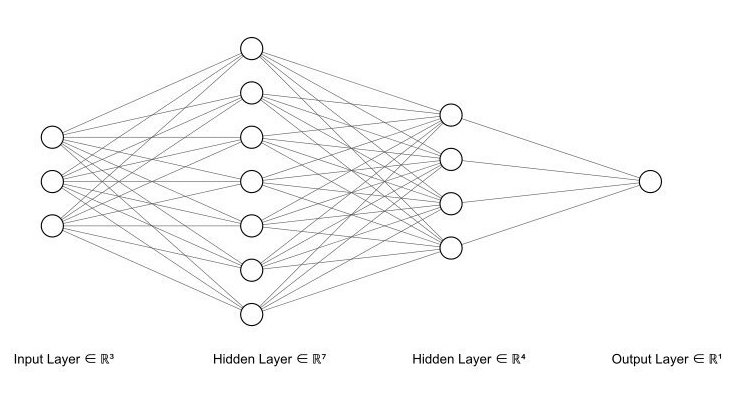
\includegraphics[width=\linewidth]{neural_net}
      \caption{A neural network with input $x\in \R^4$ and output $y\in\R^2$. The five hidden layers have dimensions $3$, $4$, $5$, $3$ and $7$ respectively. The graphic was generated with http://alexlenail.me/NN-SVG/index.html}\label{img_nn}
	\end{minipage}
\end{center}
\end{figure}


\section{Training of neural networks}\label{sec:training_of_nn}
Since we now know what neural networks are, we want to discuss how to tune them to a specific problem. This procedure is usually referred to as training of a neural network. There are many approaches of how to train a neural network (\textcolor{red}{TODO: cite some approaches then!}). However, most of them rely on iteratively finding the gradient - the direction of greatest ascent of the risk function, and afterwards performing an optimization step in the opposite of the found direction. This method of the steepest descent dates way back to the early $\nth{19}$ century and was introduced by Augustin L. Cauchy in the year $1847$. For a brief overview we refer to \cite{lemarechal2012cauchy}. This method is immensely popular and thus, can be discovered in numerous literature. We will mostly draw inspiration form \cite[Chapter~XV]{kantorovich2016functional}. For in-depth explanation, please take a look at this reference.\\
Let us consider a (non-linear) real-valued function $f$, which is defined on a real normed space $X$. We assume that $f$ is bounded below on $X$ and we aim to find an element $x^{\ast}\in X$ such that

\begin{align*}
f(x) \geq f(x^{\ast}),
\end{align*}

for all $x\in X$. Hence, $x^{\ast}$ minimizes the function $f$. To solve this problem, one usually constructs a sequence $(x_n)$ that minimizes $f$, in the sense that

\begin{align*}
\lim_{n\to\infty} f(x_n) = \inf_{x\in X} f(x).
\end{align*}

In certain cases, one can construct such a sequence such that it converges to an optimum $x^{\ast}$. If the considered function $f$ is assumed to be continuous, then this element will be a solution to the proposed problem.\\
To construct such a sequence, we assume that the function $f$ is \textbf{differentiable}. This means, that the directional derivative

\begin{align*}
\frac{\partial f}{\partial z} (x) \coloneqq \frac{1}{\|z\|} \lim_{h \to 0^+} \frac{f(x + hz) - f(x)}{h},
\end{align*}
exists at each point $x \in X$ and for every direction $z \in X$. If the function and its derivative are additionally continuous, we call it \textbf{continuously differentiable}.\\
Furthermore, we assume that there exists a direction for which the derivative takes minimum value, or in other words the direction of steepest descent. This direction is the negative direction of the gradient of $f$. If we now perform a step towards the direction of steepest descent, we completed an iteration of the so called steepest descent method - or nowadays better known as the gradient descent algorithm. This algorithm we now want to consider in detail.\\
Let $X$ be a normed space and $f:X\to \R$ be a continuously differentiable function with existing minimum at $x^{\ast}$.
Furthermore, let there be a direction of steepest descent in every $x \in X$ and $x^{(0)}\in X$ an arbitrary (initial) element. Assume that we already found the $k$-th iterate $x^{(k)}$, then we define the $(k+1)$-th iterate by

\begin{align}\label{eq:gd}
x^{(k+1)} \coloneqq x^{(k)} - \g_{k+1} z_{k+1},
\end{align}

where $z_{k+1}$ denotes the direction of steepest descent at $x^{(k)}$. The numerical parameter $\g^{(k+1)}$ can be found in various ways, e.g. \cite[Chapter~XV]{kantorovich2016functional}. However, we want to approach it by finding the optimal step size analytically.\\
We specify a sequence of positive numbers $(\g_k)$ such that $\g_k \to 0$ and $\sum_{k\geq 1} \g_k = \infty$. Furthermore, we assume the $z_k$ to be normalized for all $k\in \N$, i.e. $\|z_k\| = 1$. Hence, the step size at the $k$-th iteration is $\g_k$. We do this in order to avoid doing to great steps, which would eventually avert the convergence of the algorithm.\\
Furthermore, we note at this point that we can establish a connection between the problem of minimizing a functional and that of solving a linear functional equation as follows.\\
Let $U$ be a self-adjoint operator on a Hilbert space $\H$. We assume that the operator $U$ is below bounded by $m>0$ and above bounded by $M>0$, i.e. the following equations hold
\begin{align*}
m \coloneqq \inf_{x\in X, \|x\| = 1} \left\langle Ux, x \right\rangle, \qquad \text{and} \qquad M \coloneqq \sup_{x\in X, \|x\| = 1} \left\langle Ux, x \right\rangle,
\end{align*}
which implies that $U$ is an injective operator.\\
Now, lets consider the linear functional equation
\begin{align}\label{eq:lfe}
Ux = y.
\end{align}
Since $U$ is injective the inverse operator $U^{-1}$ exists. Therefore, there exists one unique solution to \eqref{eq:lfe}, for each $y\in\H$. Now, we define the functional
\begin{align}\label{eq:functional}
F(x) = \left\langle Ux, x\right\rangle - \left( \left\langle x, y\right\rangle + \left\langle y, x\right\rangle \right) = \left\langle Ux, x\right\rangle - 2 \left\langle x, y\right\rangle.
\end{align}
With the help of the functional \eqref{eq:functional} we can formulate the following theorem.

\begin{theorem}\label{theorem:min_lfe}
Let $\H$ be a Hilbert space. A solution $x^{\ast}\in \H$ of \eqref{eq:lfe} yields a minimum of \eqref{eq:functional}. Conversely, if \eqref{eq:functional} attains a minimum at $x^{\prime} \in \H$, then $x^{\prime}$ is a solution of \eqref{eq:lfe}, that is, $x^{\prime} = x^{\ast}$.
\end{theorem}

\begin{proof}
Since we assumed $x^{\ast} \in \H$ to be a solution of \eqref{eq:lfe}, we can express $F$ as
\begin{align}\label{eq:F_rewritten}
F(x) = \left\langle Ux, x \right\rangle - \left\langle x, Ux^{\ast} \right\rangle - \left\langle Ux^{\ast}, x \right\rangle = \left\langle U(x - x^{\ast}), x - x^{\ast} \right\rangle - \left\langle Ux^{\ast}, x^{\ast} \right\rangle.
\end{align}
Using the boundedness of $U$ we receive
\begin{align}\label{eq:1.8}
F(x) \geq m\left\langle x - x^{\ast}, x - x^{\ast} \right\rangle - \left\langle Ux^{\ast}, x^{\ast} \right\rangle &\geq - \left\langle Ux^{\ast}, x^{\ast} \right\rangle\nonumber\\
&= \left\langle Ux^{\ast}, x^{\ast} \right\rangle  -2\left\langle Ux^{\ast}, x^{\ast} \right\rangle = F(x^{\ast}).
\end{align}
That is, $x^{\ast} \in \H$ indeed minimizes the functional $F$.\\
To prove the second part of the theorem, we assume that \eqref{eq:functional} attains a minimum at $x^{\prime} \in \H$. Furthermore, we assume that $x^{\ast}\in\H$ is the solution of \eqref{eq:lfe}. Therefore, we consider the following equation
\begin{align*}
F(x^{\prime}) - F(x^{\ast}) = 0.
\end{align*}
The definition of the functional \eqref{eq:functional} gives us
\begin{align*}
F(x^{\prime}) - F(x^{\ast}) &= \left\langle Ux^{\prime}, x^{\prime}\right\rangle -  2\left\langle x^{\prime}, y\right\rangle - \left\langle Ux^{\ast}, x^{\ast}\right\rangle - 2 \left\langle x^{\ast}, y\right\rangle.
\end{align*}
Now we use the fact, that $x^{\ast}$ solves the equation \eqref{eq:lfe}
\begin{align*}
\left\langle Ux^{\prime}, x^{\prime}\right\rangle -  2\left\langle x^{\prime}, y\right\rangle - \left\langle Ux^{\ast}, x^{\ast}\right\rangle + 2 \left\langle x^{\ast}, y\right\rangle
= \left\langle Ux^{\prime}, x^{\prime}\right\rangle - 2 \left\langle x^{\prime}, Ux^{\ast}\right\rangle + \left\langle Ux^{\ast}, x^{\ast}\right\rangle.
\end{align*}
Lastly, we use the linearity of the inner product as in equation \eqref{eq:F_rewritten} and the lower bound of the operator $U$.
\begin{align*}
\left\langle Ux^{\prime}, x^{\prime}\right\rangle - 2 \left\langle x^{\prime}, Ux^{\ast}\right\rangle + \left\langle Ux^{\ast}, x^{\ast}\right\rangle &=\left\langle U(x^{\prime} - x^{\ast}), x^{\prime} - x^{\ast} \right\rangle\\
&\geq m \left\langle x^{\prime} - x^{\ast}, x^{\prime} - x^{\ast} \right\rangle,
\end{align*}
therefore, $x^{\prime} = x^{\ast}$.
\end{proof}

With the help of Theorem \ref{theorem:min_lfe} we realise that finding the solution to a linear functional equation is equivalent to minimizing the corresponding functional. Hence, we want to apply the method of steepest descent to the functional in order to find the solution of the linear functional equation. In other words, applying the method of steepest descent to a given functional gives us a sequence $(x^{(k)})$ that converges to a $x^{\ast}$, which minimizes the functional. This consideration we now want to formulate in detail.

\begin{corollary}\label{cor:gd}
Let $\H$ be a Hilbert space and $F$ be a functional as defined in \eqref{eq:functional}. Then the gradient descent algorithm applied to the functional $F$ with arbitrary initial iterate $x^{(0)}\in\H$ looks like
\begin{align*}
x^{(k)} = x^{(k-1)} - \g_{k-1}z_{k-1},
\end{align*}
where $z_k\in\H$ and $\g_k>0$ look like
\begin{align*}
z_k = Ux^{(k-1)} - y \qquad\text{and} \qquad\g_k = \frac{\langle z_k, z_k \rangle}{\langle Uz_k, z_k \rangle}.
\end{align*}
Moreover, we note that we choose an optimal step size $\g_k$ in each iteration.
\end{corollary}

\begin{proof}
Let $x, z\in \H$, then
\begin{align}\label{eq:F_dir}
F(x + z) &= \left\langle U(x + z), x + z \right\rangle - \left( \left\langle x + z, y \right\rangle + \left\langle y, x + z \right\rangle  \right)\nonumber\\
&= \left\langle Ux, x \right\rangle - \left( \left\langle x, y \right\rangle + \left\langle y, x \right\rangle  \right) + \left( \left\langle Ux - y, z \right\rangle + \left\langle z, Ux - y \right\rangle \right) + \left\langle Uz, z \right\rangle\nonumber\\
&= F(x) + \left( \left\langle Ux - y, z \right\rangle + \left\langle z, Ux - y \right\rangle \right) + \left\langle Uz, z \right\rangle.
\end{align}
Considering the derivative in direction $z$ gives us
\begin{align*}
\frac{\partial F}{\partial z} (x) = \frac{1}{\|z\|} \left(  \left\langle Ux - y, z \right\rangle + \left\langle z, Ux - y \right\rangle \right) = \frac{2 \langle Ux - y, z \rangle}{\|z\|},
\end{align*}
where in the last equation we used the fact that $F$ is a real-values function.\\
Thus the direction of steepest ascent at $x^{(0)}\in\H$ is given by $z_1 = Ux^{(0)} - y$ and the direction of steepest descent by $-z_1$.\\
Lastly, to determine the descent value we want to introduce the concept of rays, emanating of a point $x\in \H$ in direction $z\in\H$. This is the set of elements that is generated by $x + \a z$, where $\a>0$ is a non-negative real number and $z\in\H$ is the direction of the ray. The restriction of the function $F$ onto this ray is thereby a function of a real variable that we will denote as $f(\a; x, z) = F(x + \a z)$ for $\a \geq 0$.\\
We consider the ray emanating of our current iterate $x^{(0)}$ in the direction of the steepest descent $z_1$ and consider it as a real valued function in $\a$. Since we want to find an optimal descent value, we look for the minimum on this ray, what ultimately results in a one dimensional optimization problem. Hence, we consider the equation
\begin{align}\label{eq:deriv_cond}
\frac{\partial f(\a; x^{(0)}, - z_1)}{\partial \a} = 0,
\end{align}
where with the use of equation \eqref{eq:F_dir}, we have
\begin{align*}
f(\a; x^{(0)}, -z_1) = F(x^{(0)} - \a z_1) = F(x^{(0)}) - 2 \a\left\langle z_1, z_1 \right\rangle + \a^2\left\langle Uz_1, z_1 \right\rangle.
\end{align*}
Thus, the derivative $\partial f(\a; x^{(0)}, - z_1)/\partial \a$ looks like
\begin{align*}
\frac{\partial f(\a; x^{(0)}, - z_1)}{\partial \a} = - 2\left\langle z_1, z_1 \right\rangle + 2\a\left\langle Uz_1, z_1 \right\rangle.
\end{align*}
Considering the condition \eqref{eq:deriv_cond} gives us the descent value by solving for $\a$
\begin{align*}
\Longleftrightarrow \qquad  2\left\langle z_1, z_1 \right\rangle &= 2\a\left\langle Uz_1, z_1 \right\rangle\\
\Longleftrightarrow \qquad \frac{\left\langle z_1, z_1 \right\rangle}{\left\langle Uz_1, z_1 \right\rangle} &= \a.
\end{align*}
Therefore, by defining $\g_1 = \a$ we receive the optimal descent value in the direction $z_1$.\\
In exactly the same way $\g_k$ and $z_k$ can be determined for all $k>1$ and hence, all assertions from the theorem are proven.
\end{proof}

The gradient descent algorithm with parameters as asserted in Corollary \ref{cor:gd} does converge, as we have seen in the proof. However, one might pose the question how quickly it converges. This question we want to consider in the following theorem.

\begin{theorem}\label{theorem:gd}
Let the same assumptions as in Corollary \ref{cor:gd} hold. Then the constructed sequence $(x^{(n)})$ with $(z_n), (\g_n)$ as in Corollary \ref{cor:gd}, converges to $x^{\ast}\in\H$. Its speed of convergence is given by
\begin{align*}
\left\|x^{(n)} - x^{\ast}\right\| \leq \frac{\|z_1\|}{m}\left( \frac{M - m}{M + m} \right)^n,
\end{align*}
for all $n\in\N_0$.
\end{theorem}

\begin{proof}
Firstly, we rewrite the equation \eqref{eq:lfe} with $k>0$ to
\begin{align}\label{eq:rewritten}
Ux &= y\nonumber\\
\Longleftrightarrow \qquad 0 &= ky - kUx\nonumber\\
\Longleftrightarrow \qquad x &= x - kUx + ky.
\end{align}
We chose the numerical factor $k$ in a way, that the operator $T=\id-kU$ has the smallest possible norm, where we denote $\id$ as the identity operator. Since we assumed $U$ to be lower bounded by $m$ and upper bounded by $M$, the operator $T$ needs to be lower bounded by $1-km$ and upper bounded by $1-kM$, where the minimal norm will occur if
\begin{align*}
1-km = -(1-kM).
\end{align*}
This leads to
\begin{align*}
k = \frac{2}{m + M}.
\end{align*}
Therefore, for $\|T\|$ it holds
\begin{align}\label{eq:lower}
\|T\| = 1 - km = 1 - \frac{2m}{m+M},
\end{align}
as well as
\begin{align}\label{eq:upper}
\|T\| = kM - 1 = \frac{2M}{m+M} - 1.
\end{align}
Combining the equations \eqref{eq:lower} and \eqref{eq:upper} leads to
\begin{align*}
2\|T\| &= \left( 1 - \frac{2m}{m+M}\right) + \left( \frac{2M}{m+M} - 1\right) = \frac{2M - 2m}{m+M}\\
\Longleftrightarrow \qquad \|T\| &= \frac{M-m}{M+m}.
\end{align*}
Moreover, applying \eqref{eq:rewritten} and rewriting it gives us
\begin{align}\label{eq:x_prime}
x^{\prime}_1 = Tx^{(0)} + ky = x^{(0)} - k(Ux^{(0)} - y) = x^{(0)} - kz_1.
\end{align}
Let us introduce the operator $V = U^{1/2}$, which is the root operator of $U$, see e.g \cite[Theorem~V.6.2]{kantorovich2016functional}. This is the unique operator that fulfils the equation $V^2 = U$. Furthermore, we should not that the operator $V$ indeed exists due to the fact that $U$ is a self-adjoint and hence positive operator. The same properties then hold for the operator $V$ as well.\\
This operator $V$ we now plug into \eqref{eq:F_rewritten}.
\begin{align}\label{eq:F_rewritten2}
F(x) &= \left\langle U(x - x^{\ast}), x - x^{\ast} \right\rangle - \left\langle Ux^{\ast}, x^{\ast} \right\rangle\nonumber\\
&= \left\langle V(x - x^{\ast}), V(x - x^{\ast}) \right\rangle - \left\langle Vx^{\ast}, Vx^{\ast} \right\rangle\nonumber\\
&= \left\|V(x - x^{\ast}) \right\|^2 - \left\|Vx^{\ast} \right\|^2
\end{align}
Considering the inequality $F(x^{\prime}_1) \geq F(x^{(1)})$, which holds due to the fact that $x^{(1)}$ is the iterate performed with optimal descent value, leads to
\begin{align*}
F(x^{(1)}) -F(x^{\ast}) \leq F(x^{\prime}_1) -F(x^{\ast}),
\end{align*}
which we can rewrite again with the use of \eqref{eq:F_rewritten2}
\begin{align}\label{ineq:1}
\left\| V(x^{(1)} - x^{\ast}) \right\| \leq \left\| V(x^{\prime}_1 - x^{\ast}) \right\|.
\end{align}
Since equation \eqref{eq:F_rewritten} was the rewritten equation \eqref{eq:lfe}, we can write with the definition of $T$
\begin{align*}
x^{\ast} = Tx^{\ast} + ky,
\end{align*}
subtracting this equation from \eqref{eq:x_prime} gives us
\begin{align*}
x^{\prime}_1 - x^{\ast} = T(x^{(0)} - x^{\ast}),
\end{align*}
applying the operator $V$ on both sides gives us
\begin{align}\label{eq:1.16}
V\left(x^{\prime}_1 - x^{\ast}\right) = VT(x^{(0)} - x^{\ast}).
\end{align}
With the easy calculation
\begin{align*}
VT = V\left( I - kU\right) = V -kVU = V - kVVV = \left(I-kU\right)V = TV,
\end{align*}
we realise that the operators $T$ and $V$ commute. Hence, we can rewrite \eqref{eq:1.16} to
\begin{align*}
V\left(x^{\prime}_1 - x^{\ast}\right) = TV(x^{(0)} - x^{\ast}).
\end{align*}
Considering the norm leads to
\begin{align*}
\left\|V\left(x^{\prime}_1 - x^{\ast}\right)\right\| &= \left\| TV(x^{(0)} - x^{\ast})\right\| \leq \left\| T \right\| \left\|V(x^{(0)} - x^{\ast})\right\|\\
&=\frac{M-m}{M+m} \left\|V(x^{(0)} - x^{\ast})\right\|\\
\end{align*}
Therefore, with inequality \eqref{ineq:1} we have
\begin{align*}
\left\| V(x^{(1)} - x^{\ast}) \right\|\leq \frac{M-m}{M+m} \left\|V(x^{(0)} - x^{\ast})\right\|.
\end{align*}
If we apply exactly the same arguments for all $k\in\{1,\ldots n\}$, then we have the following bound for the $n$-th iterate
\begin{align*}
\left\| V(x^{(n)} - x^{\ast}) \right\|\leq \frac{M-m}{M+m} \left\|V(x^{(n-1)} - x^{\ast})\right\|,
\end{align*}
which leads to the bound
\begin{align*}
\left\| V(x^{(n)} - x^{\ast}) \right\|\leq \left(\frac{M-m}{M+m}\right)^n \left\|V(x^{(0)} - x^{\ast})\right\|.
\end{align*}
Furthermore, we realise that the function $t^{-1/2}$ is continuous in $[m, M]$ and therefore especially on the spectrum of $U$, which leads to the observation that the inverse operator $U^{-1/2} = V^{-1}$ exists.\\
Moreover, with the help of \cite[Theorem~V.6.2]{kantorovich2016functional} (which regards the spectrum $S_U$ of the operator $U$) the following equations hold
\begin{align*}
\left\|V^{-1}\right\| &= \max_{t\in S_U} \frac{1}{\sqrt{t}} = \frac{1}{\sqrt{m}},\\
\left\|V\right\| &= \max_{t\in S_U} \sqrt{t} = \sqrt{M}.
\end{align*}
Combining the above results, we receive
\begin{align}\label{eq:combined}
\left\| x^{(n)} - x^{\ast} \right\| = \left\| V^{-1}V\left(x^{(n)} - x^{\ast}\right) \right\|&\leq \left\| V^{-1}\right\| \left\|V\left(x^{(n)} - x^{\ast}\right) \right\|\nonumber\\
&\leq \left\| V^{-1}\right\|\left( \frac{M-m}{M+m} \right)^n \left\|V\left(x^{(0)} - x^{\ast}\right) \right\|\nonumber\\
&\leq \frac{1}{\sqrt{m}}\left( \frac{M-m}{M+m} \right)^n \left\|V\left(x^{(0)} - x^{\ast}\right) \right\|.
\end{align}
However, since the unknown element $x^{\ast}$ appears on the right-hand side, we want to somehow remove it. In order to do this, we consider
\begin{align*}
\left\|V(x^{(0)} - x^{\ast}) \right\| = \left\|V^{-1}U(x^{(0)} - x^{\ast}) \right\| \leq \left\|V^{-1}\right\| \left\|U(x^{(0)} - x^{\ast}) \right\| = \frac{\|z_1\|}{\sqrt{m}}.
\end{align*}
Plugging this result into \eqref{eq:combined}, gives us
\begin{align*}
\left\| x^{(n)} - x^{\ast} \right\| \leq \frac{\|z_1\|}{m}\left( \frac{M-m}{M+m} \right)^n.
\end{align*}
This is exactly the inequality asserted in the theorem.
\end{proof}

As we saw in  Theorem \ref{theorem:gd} the gradient descent algorithm does converge, we even determined an upper bound to its convergence speed. However, the algorithm relies on computing the gradient of the function to be optimized. In our setting, this is the gradient of the risk function that has a neural network as prediction function, where the gradient is computed with regard to the parameters of the neural network. Since it is unclear how such a gradient actually looks like, we want to consider some examples.

\begin{example}\label{ex:nn_gradients_1dim}
Let's first consider the easiest neural network possible, two connected neurons. Afterwards, we want to generalize this to a neural network that consists of $L\in\N$ layers, where each layer does only have one neuron. Lastly, we will consider a neural network with two hidden layers, where there are $d_1>1$ and $d_2>1$ neurons in the first and second layer, respectively. Moreover, let $\f$ be the sigmoid activation function, $D$ be an arbitrary dataset of length $d\in\N$ and $\loss$ be the mean squared error loss, see Example \ref{ex:supervised_loss}.
\begin{enumerate}
\item We consider a neural network $f$, that consists of an input neuron and an output neuron. Hence, we can describe it as
\begin{align}\label{eq:nn1}
f(x) = \f\left(wx + b\right) \qquad x\in\R,
\end{align}
where $w\in\R$ is the networks weight and $b\in\R$ is the networks bias.\\
Since we are interested in computing the gradient of the empirical risk function, we want to formulate it explicitly.
\begin{align*}
\risk_{\loss, D} (f_\t) = \frac{1}{d} \sum_{i=1}^d \left| y_i - f(x_i)\right|^2.
\end{align*}
Plugging in the explicit definition of the neural network from equation \eqref{eq:nn1}, gives us
\begin{align}\label{eq:risk_expl}
\risk_{\loss, D} (f_\t) = \frac{1}{d} \sum_{i=1}^d \left| y_i - (\f(wx_i) + b ) \right|^2.
\end{align}
Now, lets consider how the gradient of \eqref{eq:risk_expl} with regard to the parameters $\t=(w, b)$ of the neural network $f_{\t}$ looks like. In mathematical notation, this means $\partial \risk_{\loss, D}(f_w)/\partial w$.\\
However, since the empirical risk function is the mean of loss functions, the gradient of the empirical risk function is the mean of the gradients of the loss functions as well. Hence, we need to compute $\partial \loss(f_{\t}, y)/\partial \t$.\\
At this point, we want to remember the chain rule of differentiation, see e.g. \cite[Chapter19.6]{simmons1995calculus} which states
\begin{align}\label{eq:chain_rule}
\frac{\partial f(g(x))}{\partial x} = \frac{\partial g(x)}{\partial x} \frac{\partial f(g(x))}{\partial g(x)}.
\end{align}
With the help of the chain rule, we can compute the gradient of the loss function by computing it as
\begin{align}\label{eq:loss_expl}
\frac{\partial \loss(f_\t(x), y)}{\partial \t} = \frac{\partial \loss(f_\t(x), y)}{\partial f_\t(x)}\frac{\partial f_\t(x)}{\partial \t}.
\end{align}
This expression we can compute easily, since $\partial f_\t(x)/\partial \t$ is
\begin{align*}
\frac{\partial f_\t(x)}{\partial \t}
&= \left[\frac{\partial (\f(wx) + b)}{\partial w}, \frac{\partial (\f(wx) + b)}{\partial b} \right]^{\tran}\\
&= \left[\frac{\partial (\f(wx) + b)}{\partial wx} \frac{\partial wx}{\partial w}, \frac{\partial (\f(wx) + b)}{\partial b} \right]^{\tran} = \left[x\f^{\prime}(x), 1 \right]^{\tran},
\end{align*}
where the derivative of the sigmoid function is $\f^{\prime}(x) = \f(x)(1 - \f(x))$.\\
Furthermore, the second part $\partial \loss(f_w(x), y)/\partial f_w(x)$ of the right-hand side \eqref{eq:loss_expl} is
\begin{align*}
\frac{\partial \loss(f_\t(x), y)}{\partial f_\t(x)} = \frac{\partial |f_\t(x) - y|^2}{\partial f_\t(x)} = 2 \left(f_\t(x) + b - y \right) = 2 \left(\f(wx) + b - y \right).
\end{align*}
Therefore, plugging this into equation \eqref{eq:loss_expl}, we receive
\begin{align*}
\frac{\partial \loss(f_\t(x), y)}{\partial \t} &= 2 \left(\f(wx) + b - y \right) \f^{\prime}(x) \left[x\f^{\prime}(x), 1 \right]^{\tran}\\
&= 2 \left[ \begin{matrix}
x(\f^{\prime}(x))^2\left(\f(wx) + b - y \right)\\
\left(\f(wx) + b - y \right) \f^{\prime}(x)
\end{matrix}
\right].
\end{align*}
Lastly, we can insert the data samples $(x, y)\in D$ to compute the gradient of the empirical risk function. This leads to
\begin{align*}
\nabla_{\t} \risk_{\loss, D} (f_{\t}) = \frac{2}{d} \sum_{(x,y)\in D} \left[ \begin{matrix}
x(\f^{\prime}(x))^2\left(\f(wx) + b - y \right)\\
\left(\f(wx) + b - y \right) \f^{\prime}(x)
\end{matrix}
\right].
\end{align*}
\item Since neural networks usually consist of more than two neurons, we now want to consider how we can generalize the neural network to a more complex architecture.\\
Let $L\in\N$ and $L+1$ denote the number of layers in the neural network, where each layer consist of one neuron. Hence for each $i=1,\ldots, L$ holds
\begin{align*}
H_i: \R &\to \R,\\
x &\mapsto \f\left(wx_i + b_i\right).
\end{align*}
For simplicity reasons, we assume that $\f=\id$ and $b_i=0$ for all $i=1,\ldots L$. Otherwise, the computation would be the same as in the first example. Therefore, we can denote the neural network as
\begin{align*}
f_\t(x) = H_L \circ \ldots \circ H_1(x) = H_L(H_{L-1}(\ldots(H_1(x))\ldots) \qquad x\in\R,
\end{align*}
where $\t=(\t_1,\ldots,\t_L)$ denotes the parameters of the neural network. Since we assumed $b_i=0$ for all $i=1,\ldots L$, we can denote the parameters as $\t=(w_1,\ldots w_L)$.\\
Our goal is to compute the gradient of the empirical risk function, what we can do by computing the gradient of the loss function, analogously to the first example. However, instead of considering the whole vector $\t$ at once, we want to compute the gradient for each parameter $\t_i=w_i$ separately, since for the gradient holds
\begin{align*}
\nabla_\t \loss (f_{\t}(x), y) = \left[\begin{matrix}
\nabla_{w_1}\loss (f_{\t}(x), y)\\
\vdots\\
\nabla_{w_L}\loss (f_{\t}(x), y)
\end{matrix} \right].
\end{align*}
To compute the gradients, we start at the last layer and iteratively compute the parameters of the preceding layer. This method is well known as back-propagation, which we will define more general after considering this comparatively easy example.\\
As already described, we want to start by computing $\partial \loss (f_{\t}(x), y) / \partial w_L$. Considering the chain rule from equation \eqref{eq:chain_rule}, we receive
\begin{align*}
\frac{\partial \loss (f_{\t}(x), y)}{ \partial w_L} = \frac{\partial \loss (f_{\t}(x), y)}{\partial f_{\t}(x)} \frac{\partial f_{\t}(x)}{ \partial w_L}.
\end{align*}
At this point, we want to define $x^{(i)}\coloneqq H_i(x)$ for all $i=1,\ldots L$, where $x|in\R^{i-1}$. With this definition we can write $f_{\t}(x) = H_L(x^{(L-1)})$ and therefore,
\begin{align}\label{eq:grad_split}
\frac{\partial \loss (f_{\t}(x), y)}{ \partial w_L} = \frac{\partial \loss (f_{\t}(x), y)}{\partial f_{\t}(x)} \frac{\partial H_L(x^{(L-1)}}{ \partial w_L}.
\end{align}
As the next step, we want to consider both quantities of the right-hand side of \eqref{eq:grad_split} separately. The first part $\partial \loss (f_{\t}(x), y) / \partial f_{\t}(x)$ results to be
\begin{align*}
\frac{\partial \loss (f_{\t}(x), y)}{\partial f_{\t}(x)} = \frac{\partial (f_{\t}(x) - y)^2}{\partial f_{\t}(x)} = 2 (f_{\t}(x) - y),
\end{align*}
and for the second part $\partial H_L(x^{(i-1)}) /\partial w_L$ holds
\begin{align*}
\frac{\partial H_L(x^{(i-1)})}{ \partial w_L} = \frac{\partial w_Lx^{(L-1)}}{ \partial w_L} = x^{(L-1)} = x\prod_{i=1}^{L-1} w_i.
\end{align*}
Therefore, plugging the two results into \eqref{eq:grad_split} gives us
\begin{align*}
\frac{\partial \loss (f_{\t}(x), y)}{ \partial w_L} = 2x (f_{\t}(x) - y) \prod_{i=1}^{L-1} w_i.
\end{align*}
Doing this for all $i=1,\ldots, L-1$ gives us for the parameters $w_i$
\begin{align*}
\frac{\partial \loss (f_{\t}(x), y)}{ \partial w_i} = \frac{\partial \loss (f_{\t}(x), y)}{\partial f_{\t}(x)} \frac{\partial H_i(x^{(i-1)}}{ \partial w_i},
\end{align*}
where we define $x^{(0)} \coloneqq x$. Hence, we receive for $i=2,\ldots,L$
\begin{align*}
\frac{\partial \loss (f_{\t}(x), y)}{ \partial w_i} = 2x (f_{\t}(x) - y) \prod_{k=1}^{i-1} w_k.
\end{align*}
Considering the case $i=1$ separately, gives us
\begin{align*}
\frac{\partial \loss (f_{\t}(x), y)}{ \partial w_1} &= \frac{\partial \loss (f_{\t}(x), y)}{\partial f_{\t}(x)} \frac{\partial H_1(x^{(0)}}{ \partial w_1}\\
&= \frac{\partial  (f_{\t}(x) - y)^2}{\partial f_{\t}(x)} \frac{\partial w_1x}{ \partial w_1} = 2x (f_{\t}(x) - y).
\end{align*}
Combining the computed gradients gives us the desired gradient of the loss function
\begin{align*}
\nabla_\t \loss (f_{\t}(x), y) = \left[\begin{matrix}
2x (f_{\t}(x) - y)\\
2x (f_{\t}(x) - y) w_1\\
\vdots\\
2x (f_{\t}(x) - y) \prod_{k=1}^{L-1} w_k
\end{matrix} \right].
\end{align*}
Lastly, we remember that the gradient of the empirical risk function is the mean of gradients of the loss function. Hence, the gradient of the empirical risk function with reard to the parameters of the neural network looks like
\begin{align*}
\nabla_{\t}\risk_{\loss, D} (f_{\t}) = \frac{2}{d} \sum_{(x, y)\in D} \left[\begin{matrix}
x (f_{\t}(x) - y)\\
x (f_{\t}(x) - y) w_1\\
\vdots\\
x (f_{\t}(x) - y) \prod_{k=1}^{L-1} w_k
\end{matrix} \right].
\end{align*}
\iffalse
\item The last example we want to consider is a neural network with an input layer of dimension $d_i\in\N$, an output layer of dimension $d_o\in\N$ and a hidden layer of dimension  $d_h\in\N$. Furthermore, we assume $d_i, d_o, d_h > 1$. Therefore the first layer looks like
\begin{align*}
H_1: \R^{d_i} &\to \R^{d_h},\\
x &\mapsto W_1x + b_1,
\end{align*}
where $b_1\in\R^{d_h}$ and $W_1\in\R^{d_h}\times\R^{d_i}$, and the second layer looks like
\begin{align*}
H_2: \R^{d_h} &\to \R^{d_o},\\
x &\mapsto W_2x + b_2,
\end{align*}
where $b_2\in\R^{d_o}$ and $W_2\in\R^{d_o}\times\R^{d_h}$.\\
Moreover, we consider the activation function to be $\f=\id$ and the biases be $0$. The neural network then results to look like
\begin{align*}
f_{\t}(x) = H_2 \circ H_1 (x) = H_2(H_1(x)) = W_2 W_1 x,
\end{align*}
where $\t = (W_1, W_2)$.\\
Let $f_{\t}(x)_i$ denote the $i$-th coordinate of $f_{\t}(x)$, then the loss function $\loss$ looks like
\begin{align*}
\loss(f_{\t}(x), y) = \sum_{i=1}^{d_o}\left| f_{\t}(x)_i - y_i \right|^2 = \sum_{i=1}^{d_o}\left| (W_2 W_1 x)_i - y_i \right|^2.
\end{align*}
Deriving the loss function with regard to the weights, gives us with the chain rule from equation \eqref{eq:chain_rule}
\begin{align}\label{eq:loss_chained}
\frac{\partial \loss(f_{\t}(x), y)}{\partial \t} = \frac{\partial \loss(f_{\t}(x), y)}{\partial f_{\t}(x)} \frac{\partial f_{\t}(x)}{\partial \t}.
\end{align}
However, since we find ourselves in the multidimensional setting we need to introduce a well known quantity from calculus, the Jacobian matrix. Let $f:\R^n \to \R^m$ be a function that looks like $f(x) = [f_1(x_1,\ldots,x_n), \ldots, f_m(x_1,\ldots,x_n)]$. Then its derivative is called \textbf{Jacobian matrix} and looks like
\begin{align}\label{eq:Jacobian}
\frac{\partial f}{\partial x} = \left[
\begin{matrix}
&\frac{\partial f_1}{\partial x_1} &\cdots &\frac{\partial f_1}{\partial x_n}\\
&\vdots & \ddots &\vdots\\
&\frac{\partial f_m}{\partial x_1} &\cdots &\frac{\partial f_m}{\partial x_n}
\end{matrix}.
\right]
\end{align}
With the help of the Jacobian matrix from equation \eqref{eq:Jacobian} we can compute the derivatives on the right-hand side of equation \eqref{eq:loss_chained}, but we want to consider them separately.\\
Let $f_\t(x)_i$ denote the $i$-th coordinate of $f_\t(x)$. Then the Jacobian of $\loss(f_{\t}(x), y)$ with regard to $f_{\t}(x)$ looks like
\begin{align*}
\frac{\partial \loss(f_{\t}(x), y)}{\partial f_{\t}(x)} =
\left[\begin{matrix}
\displaystyle\frac{\partial \loss(f_{\t}(x), y)}{\partial f_{\t}(x)_1}\; \cdots\; \frac{\partial \loss(f_{\t}(x), y)}{\partial f_{\t}(x)_{d_o}}
\end{matrix} \right],
\end{align*}
since the loss function $\loss$ maps from $\R^{d_o}$ to $\R$.\\
Now we want to consider the second term of the right-hand side of \eqref{eq:loss_chained}. First of, we realise that the neural network $f_{\t}$ maps from $\R^{d_i}$ to $\R^{d_o}$. Therefore, we need to use the multi-variable chain rule, see e.g. \cite{simmons1995calculus}. This means that if we have a function in two variables $f(x,y)$, where we define $x=g(t)$ and $y=h(t)$ that the derivative $\partial f/\partial t$ looks as follows
\begin{align}\label{eq:multi_chain}
\frac{\partial f}{\partial t} = \frac{\partial f}{\partial x} \frac{\partial x}{\partial t} + \frac{\partial f}{\partial y} \frac{\partial y}{\partial t}.
\end{align}
Applying this to our setting, where we have the neural network $f_{\t}$, which ultimately is a function in $d_o$ variables. Let $f_{\t}(x)_i$ denote the $i$-th coordinate of $f_{\t}(x)$,
hence we can write $f_{\t}(x) = [f_{\t}(x)_1, \ldots f_{\t}(x)_{d_o}]$. Furthermore, we realise that for each $i=1,\ldots,d_o$ holds
\begin{align*}
f_{\t}(x)_i = W_{2,i} W_1(x) \qquad x\in \R^{d_i},
\end{align*}
where we define $W_{2,i}$ as the $i$-th row of the matrix $W_2$. Analogously, we define $H_{2,i}(x) = W_{2,i}x$ for $x\in\R^{d_h}$. Hence, we can write
\begin{align*}
f_{\t}(x) = \left[H_{2,1}(z), \ldots H_{2,d_o}(z) \right],
\end{align*}
with $z\coloneqq H_1(x)$, to simplify the notation. If we now apply the multi-variable chain rule from equation \eqref{eq:multi_chain}, we receive
\begin{align*}
\frac{\partial f_{\t}}{\partial \t} = \sum_{i=1}^{d_o} \frac{\partial f_{\t}}{\partial H_{2,i}} \frac{\partial H_{2,i}}{\partial \t}.
\end{align*}
However, we realise that for each $i=1,\ldots d_o$ we can represent $H_{2,i}(z)$ again as a function in $d_h$ variables. Hence, we can write
\begin{align*}
H_{2,i}(z) = \left[H_{1,1}(x), \ldots H_{1,d_h}(x) \right], \qquad x\in\R^{d_i}.
\end{align*}
Therefore, we can apply the multi-variable chain rule again and receive
\begin{align*}
\frac{\partial f_{\t}}{\partial \t} = \sum_{i=1}^{d_o} \frac{\partial f_{\t}}{\partial H_{2,i}} \frac{\partial H_{2,i}}{\partial \t} = \sum_{i=1}^{d_o} \sum_{j=1}^{d_h} \frac{\partial f_{\t}}{\partial H_{2,i}} \frac{\partial H_{2,i}}{\partial H_{1,j}}
\frac{\partial H_{1,j}}{\partial \t}.
\end{align*}
One may realise that as soon as the architecture of the neural network becomes more and more complex, as does the computation of the gradient. For this case, where we only have one hidden layer and one output layer the gradient of the loss function results to
\begin{align*}
\frac{\partial \loss(f_{\t}(x), y)}{\partial \t} = \left[\begin{matrix}
\displaystyle\frac{\partial \loss(f_{\t}(x), y)}{\partial f_{\t}(x)_1}\; \cdots\; \frac{\partial \loss(f_{\t}(x), y)}{\partial f_{\t}(x)_{d_o}}
\end{matrix} \right] \cdot \sum_{i=1}^{d_o} \sum_{j=1}^{d_h} \frac{\partial f_{\t}}{\partial H_{2,i}} \frac{\partial H_{2,i}}{\partial H_{1,j}}
\frac{\partial H_{1,j}}{\partial \t}.
\end{align*}
Since we are actually interested in the gradient of the empirical risk function with regard to the dataset $D$ of length $d$, we can compute the said gradient by
\begin{align*}
\nabla_{\t} \risk_{\loss, D} (f_{\t}) = \sum_{(x, y)\in D} \left[\begin{matrix}
\displaystyle\frac{\partial \loss(f_{\t}(x), y)}{\partial f_{\t}(x)_1}\; \cdots\; \frac{\partial \loss(f_{\t}(x), y)}{\partial f_{\t}(x)_{d_o}}
\end{matrix} \right] \cdot \sum_{i=1}^{d_o} \sum_{j=1}^{d_h} \frac{\partial f_{\t}}{\partial H_{2,i}} \frac{\partial H_{2,i}}{\partial H_{1,j}}
\frac{\partial H_{1,j}}{\partial \t} (x)
\end{align*}
\fi
\end{enumerate}
\end{example}

We just saw an example of the gradient of an empirical risk function, where the prediction function is a (deep) neural network in Example \ref{ex:nn_gradients_1dim}. However, we only considered the layers to have one single neuron. Naturally, in practice neural networks rarely have layers with merely one neuron. This generalization we now want to consider. But firstly, we note that the computation of the gradient relied on the chain rule, well known in calculus. Since we now want to generalize the layers to have more than one neuron, we need to extend the chain rule to multiple dimensions. It is then called multi-variable chain rule. This result is fundamental to the immensely popular back-propagation algorithm, which is often used in scenarios where one needs to compute the gradient of a function.

\begin{theorem}\label{theorem:multi_var_chainrule}
Let $n,m\in\N$ and $f:\R^{n} \to \R$ and $g:\R^{m} \to \R^{m}$ be differentiable functions. Furthermore, we define $y \coloneqq g(x)$ and $z=f(y)$, then the \textbf{multi-variable chain rule} states that the following holds
\begin{align*}
\frac{\partial z}{\partial x_i} = \sum_{j\geq 1} \frac{\partial z}{\partial y_j} \frac{\partial y_j}{\partial x_i}.
\end{align*}
In vector notation this can be equivalently expressed as
\begin{align*}
\nabla_x z = \left( \frac{\partial y}{\partial x} \right)^{\tran} \nabla_{y} z,
\end{align*}
where $\partial y/\partial x$ is the $n\times m$ Jacobian matrix of $g$.
\end{theorem}

At this point, we want to note that the chain rule can even be extended from vectors to tensors. This is very interesting, since in many Machine Learning settings the proposed neural networks operate on tensors. However, we do not want to consider this in depth and rather refer to \cite[Chapter~6.5.2]{goodfellow2016deep}.\\
Returning to the theory we want to consider, with the help of the multi-variable chain rule which we introduced in Theorem \ref{theorem:multi_var_chainrule} we can compute the gradients of empirical risk functions, where the corresponding neural network has arbitrary size of layers.\\
The back-propagation algorithm as already described, is in its fundamental idea simple. Since the weights in each layer of the neural network depend on all the consecutive weights, we start computing the gradients for all weights in the last layer and iteratively work our way through the previous layers, until we computed the gradients for every weight. However, formulating this idea formally correct is quite messy. Therefore, we want to introduce some quantities beforehand. We know that each layer $H_i$ looks like
\begin{align*}
H_i: \R^{d_{i-1}} &\to \R^{d_{i}},\\
x &\mapsto H_i(x) = \f(W_ix + b_i),
\end{align*}
where $d_i$ describes the output dimension of the $i$-th layer and $d_{i-1}$ describes the input dimension of the $i$-th layer, as we defined in Definition \ref{def:layer}. In the following we want to denote the weight matrix as $W^{(i)}\coloneqq W_i$, since we will need the index otherwise. Furthermore, we want to denote the weight matrix as $W^{(i)} = (w^{(i)}_{jk})$, where each of the entries $w^{i}_{jk}$ describes the weight between the $k$-th neuron in the $(i-1)$-th layer and the $j$-th neuron in the $i$-th layer. With these considerations we can write the input to the $j$-th neuron of the $i$-th layer, which we want to denote as $z_{j}^{(i)}$, as
\begin{align*}
z_{j}^{(i)} = \sum_{k=1}^{d_{i-1}} w^{(i)}_{jk} \f (z_{k}^{(i-1)}) + b_j^{(i)},
\end{align*}
where $b_j^{(i)}$ denotes the $j$-th entry of the bias in the $i$-th layer.\\
To simplify the notation even more, we will denote $a_{j}^{(i)} = \f (z_{j}^{(i)})$. We note that the $z_{j}^{(i)}$ are defined in such a way that they describe the output of a neuron before applying the activation function and the $a_{j}^{(i)}$ are defined so that they describe the output of a neuron after applying the activation function. Hence, we will call this quantity the \textbf{activation} of the $j$-th neuron in the $i$-th layer.\\
Moreover, we note that the gradient of the risk function, which is the mean of gradients of the loss function with regard to the parameters of the neural network $\t$, can be denoted as follows
\begin{align*}
\nabla_\t \risk_{\loss, D} (f_{\t}) = \left[ \begin{matrix}
\nabla_{\t_{1}} \risk_{\loss, D} (f_{\t})\\
\vdots\\
\nabla_{\t_{L}} \risk_{\loss, D} (f_{\t})\\
\end{matrix}\right],
\end{align*}
where again the gradients $\nabla_{\t_{i}} \risk_{\loss, D} (f_{\t})$ can be expressed as a vector of gradients with regard to the weights and biases of the $i$-th layer.\\
With the above considerations we can compute the gradients of the risk function in each parameter. However, the computation is slightly different in the output layer and in the hidden layers. First, we want to consider the gradients for the output layer. We know that if we consider the mean squared error loss $\loss$ for an arbitrary data sample $(x,y)$ the loss function looks like
\begin{align}\label{eq:nn_loss}
\loss(y, f(x)) = \sum_{j=0}^{d_L-1} \left(a_{j}^{(L)} - y_j \right)^2,
\end{align}
such that it is the squared sum over all entries of the output vector, which is the activation vector of the last layer $a^{(L)} \coloneqq (a^{(L)}_1, \ldots, a^{(L)}_{d_L})$.
Moreover, we consider $\nabla_{\t_{L}} \risk_{\loss, D} (f_{\t})$ as the vector of gradients
\begin{align*}
\nabla_{\t_{L}} \risk_{\loss, D} (f_{\t}) = \left[\begin{matrix}
\nabla_{w^{(L)}_{11}} \risk_{\loss, D} (f_{\t})\\
\vdots\\
\nabla_{w^{(L)}_{jk}} \risk_{\loss, D} (f_{\t})\\
\nabla_{b^{(L)}_{1}} \risk_{\loss, D} (f_{\t})\\
\vdots\\
\nabla_{b^{(L)}_{j}} \risk_{\loss, D} (f_{\t})
\end{matrix} \right].
\end{align*}
These gradients we can compute easily now. We already mentioned that the gradient of the risk function is the mean of gradients of the loss functions. Hence, we can consider the gradients of the loss functions analogously to the gradient of the risk function as
\begin{align*}
\nabla_{\t_{L}} \loss(y, f_{\t}(x)) = \left[\begin{matrix}
\nabla_{w^{(L)}_{11}} \loss(y, f_{\t}(x))\\
\vdots\\
\nabla_{w^{(L)}_{jk}} \loss(y, f_{\t}(x))\\
\nabla_{b^{(L)}_{1}} \loss(y, f_{\t}(x))\\
\vdots\\
\nabla_{b^{(L)}_{j}} \loss(y, f_{\t}(x))
\end{matrix} \right].
\end{align*}
Explicitly, the computation of these gradients looks like
\begin{align*}
\nabla_{w^{(L)}_{jk}} \loss(y, a^{(L)}) = \frac{\partial \loss(y, a^{(L)})}{\partial w^{(L)}_{jk}} = \frac{\partial \loss(y, f_{\t}(x))}{\partial a_{j}^{(L)}} \frac{\partial a_{j}^{(L)}}{\partial w^{(L)}_{jk}} = \frac{\partial \loss(y, f_{\t}(x))}{\partial a_{j}^{(L)}} \frac{\partial a_{j}^{(L)}}{\partial z_{j}^{(L)}} \frac{\partial z_{j}^{(L)}}{\partial w^{(L)}_{jk}}.
\end{align*}
Now, remembering the definition of these quantities, we can compute each of the three factors on the right-hand side. It holds then with equation \eqref{eq:nn_loss}
\begin{align}\label{eq:part1}
\frac{\partial \loss(y, a^{(L)})}{\partial a_{j}^{(L)}} = \frac{\partial \sum_{j=0}^{d_L-1} \left(a_{j}^{(L)} - y_j \right)^2}{\partial a_{j}^{(L)}} = 2(a_{j}^{(L)} - y_j).
\end{align}
For the second term holds
\begin{align}\label{eq:part2}
\frac{\partial a_{j}^{(L)}}{\partial z_{j}^{(L)}} = \frac{\partial \f(z_{j}^{(L)})}{\partial z_{j}^{(L)}} = \f^{\prime} (z_{j}^{(L)}),
\end{align}
and for the third term holds
\begin{align}\label{eq:part3}
\frac{\partial z_{j}^{(L)}}{\partial w^{(L)}_{jk}} = \frac{\partial \left(\sum_{l=1}^{d_{L-1}} w^{(L)}_{jl} a_{l}^{(L-1)} + b_j^{(L)}\right)}{\partial w^{(L)}_{jk}} = a_{k}^{(L-1)}.
\end{align}
Therefore, combining the three partial derivatives gives us the gradient. This leads to
\begin{align*}
\nabla_{w^{(L)}_{jk}} \loss(y, f_{\t}(x)) = 2(a_{j}^{(L)} - y_j) \f^{\prime} (z_{j}^{(L)})) a_{k}^{(L-1)}.
\end{align*}
At this point we want to note quickly, that if we consider the partial derivative of the risk function with respect to the biases $b_{j}^{(L)}$, only the third term of the right-hand side changes. This term we considered in equation \eqref{eq:part3}. The new partial derivative is then
\begin{align*}
\frac{\partial z_{j}^{(L)}}{\partial b^{(L)}_{j}} = \frac{\partial \left(\sum_{k=1}^{d_{L-1}} w^{(L)}_{jk} a_{k}^{(L-1)} + b_j^{(L)}\right)}{\partial b^{(L)}_{j}} = 1.
\end{align*}
With these considerations we now know how to compute the gradient of the risk function with respect to $\t_L$, the parameters of the last layer. Before proceeding to compute the gradients with respect to the remaining weights, we want to first consider what we mentioned earlier. We said that computing the gradient is slightly different in the output layer than in the previous, the hidden layers. This is due to the fact that a weight that is located in the output layer affects only the activation of one output neuron. E.g. if we consider the weight $w_{jk}^{(L)}$ which connects the $k$-th neuron of the $(L-1)$-th layer with the $j$-th neuron of the $L$-th layer, then it only affects this single output neuron. In contrast, the weights in all other previous layers, the hidden layers, affect the activations of all output neurons. Since we consider neural networks where each neuron affects all activations of the subsequent layer, it is sufficient to alter any weight in the hidden layers to affect the activation of the corresponding neuron which is attached to this weight and afterwards, this one altered activation has effect on all activations in all subsequent layers. Taking this into consideration, we can compute the gradient of the risk function with respect to the weight $w_{jk}^{(L-1)}$, which connects the $k$-th neuron of the $(L-2)$-th layer with the $j$-th neuron of the $(L-1)$-th layer. We receive
\begin{align*}
\nabla_{w^{(L-1)}_{jk}} \loss(y, a^{(L)}) = \frac{\partial \loss(y, a^{(L)})}{\partial w^{(L-1)}_{jk}}.
\end{align*}
As we described the weight $w^{(L-1)}_{jk}$ affects all activations of the output layer. Thus, applying the chain rules gives us
\begin{align*}
\frac{\partial \loss(y, a^{(L)})}{\partial w^{(L-1)}_{jk}} = \sum_{h=1}^{d_L}\frac{\partial \loss(y, a^{(L)})}{\partial a_h^{(L)}} \frac{\partial a_h^{(L)}}{\partial w^{(L-1)}_{jk}},
\end{align*}
where we sum the partial derivatives with respect to all neurons $a_h^{(L)}$ in the output layer. Applying the chain rule three more times gives us
\begin{align*}
\frac{\partial \loss(y, a^{(L)})}{\partial w^{(L-1)}_{jk}} &= \sum_{h=1}^{d_L}\frac{\partial \loss(y, a^{(L)})}{\partial a_h^{(L)}} \frac{\partial a_h^{(L)}}{\partial z_h^{(L)}} \frac{\partial z_h^{(L)}}{\partial w^{(L-1)}_{jk}},\\
&= \sum_{h=1}^{d_L}\frac{\partial \loss(y, a^{(L)})}{\partial a_h^{(L)}} \frac{\partial a_h^{(L)}}{\partial z_h^{(L)}} \frac{\partial z_h^{(L)}}{\partial a_j^{(L-1)}} \frac{\partial a_j^{(L-1)}}{\partial w^{(L-1)}_{jk}},\\
&= \sum_{h=1}^{d_L}\frac{\partial \loss(y, a^{(L)})}{\partial a_h^{(L)}} \frac{\partial a_h^{(L)}}{\partial z_h^{(L)}} \frac{\partial z_h^{(L)}}{\partial a_j^{(L-1)}} \frac{\partial a_j^{(L-1)}}{\partial z_j^{(L-1)}} \frac{\partial z_j^{(L-1)}}{\partial w^{(L-1)}_{jk}}.
\end{align*}
We realise, that the first three partial derivatives of the right-hand side are exactly the same computation as when we computed the gradient with regard to a weight that is located in the output layer. Furthermore, the last two expressions consider the effect of the altered activation of the $(L-1)$-th layer on the $L$-th, the output layer. Lastly, we want to explicitly consider the last partial derivative of the right-hand side. It holds that
\begin{align*}
\frac{\partial z_j^{(L-1)}}{\partial w^{(L-1)}_{jk}} = \frac{\partial \left(\sum_{l=1}^{d_{L-2}} w_{jl}^{(L-1)}a_l^{(L-2)} + b_j^{(L-1)}\right)}{\partial w^{(L-1)}_{jk}} = a_k^{(L-2)},
\end{align*}
which is the same result as for the output layer, see \eqref{eq:part3}. Therefore, we can apply exactly the same computation until we reach the input layer. This procedure allows us to component-wise compute the gradient $\nabla_{\t}\loss(a^{(L)}, y)$, at last. Finally, we can compute the gradient of the risk function with respect to the parameters $\t$ by averaging the gradients of the loss function over the given dataset $D$.\\
Having tackled the back-propagation algorithm we now know how to compute the gradient of the risk function with regard to the parameters of a given prediction function. However, as the back-propagation algorithm clearly shows, the computation of this gradient is highly expensive, since one has to compute the gradient for every single weight in the entire neural network, separately. A popular approach is to relax this computation by only considering the gradient in one sample (or multiple samples, we speak of a mini-batch then). We want to take a closer look at this algorithm as well. Since it is quite popular, there are many good references in literature, e.g see \cite[Chapter~13.3.2]{sra2012optimization}, \cite[Chapter~4.2]{saad2009line} and \cite{turinici2021convergence}. We will focus on the latter reference.\\
Beforehand, we need to consider the empirical risk, which we defined in Definition \ref{def:empirical_risk}. Since we take the average of the loss functions with regard to the whole data set $D$, we can denote it as an integral over the dataset $D$
\begin{align*}
\risk_{\loss, D} (f) = \frac{1}{k} \sum_{i=1}^{k} \loss\left(x_i, y_i, f(x_i)\right) = \int_{D} \loss(x,y,f(x)) d(x,y).
\end{align*}
If we now randomly choose a subset $B \subseteq D$ of length $b\in\{1,\ldots,n\}$ which we will call \textbf{mini-batch of size $b$}, we can approximate the empirical risk $\risk_{\loss, D} (f)$ through $\risk_{\loss, B} (f)$, where
\begin{align*}
\risk_{\loss,B}(f) \coloneqq \int_{B}\loss(x, y, f(x)) d(x,y).
\end{align*}
One may quickly realise, that if $b=n$, we are in the regular gradient descent setting. If one chooses to be $b=1$, i.e. the subset $B$ consisting of one single sample, then we speak of \textbf{stochastic gradient descent}, otherwise of \textbf{stochastic gradient descent with batch-size $b$}.\\
In the following, we want to summarize the data samples $\o_i=(x_i,y_i)$. Hence, we can write
\begin{align*}
\risk_{\loss,B}(f) = \int_{B}\loss(\o, f(x)) d\o.
\end{align*}
Furthermore, we remember that we essentially are interested in the setting, where $f$ is a neural network. Since the neural network $f$ has parameters $\t$, which we denoted as $f_{\t}$, we will now simplify the notation as follows
\begin{align*}
\risk_{\loss,B}(f_{\t}) = \int_{B}\loss(\o, f_{\t}(x)) d\o \eqqcolon \int_{B}\loss(\o,\t) d\o \eqqcolon \risk_{\loss,B}(\t).
\end{align*}
Our goal is to find a minimum of $\t \mapsto\risk_{\loss,B} (\t)$. We approach this problem the same way as we approached the gradient descent algorithm, where we iteratively update the parameters $\t$ to minimize the risk. Therefore, we define the update rule as follows. Lets assume we already found the $n$-th iterate $\t^{(n)}$. Now we randomly choose a sample $\o_n$ and compute its loss with regard to the current parameters $\t^{(n)}$. Afterwards, we compute the gradient of the empirical risk in the sample $\o_n$ and update the parameters. This looks like
\begin{align}\label{eq:sgd}
\t^{(n+1)} = \t^{(n)} -\g_n \nabla_{\t} \loss(\o_n,\t^{(n)}).
\end{align}
This way we define a sequence of parameters $(\t^{(n)})$, which we will show to converge to some $\t^{\ast}$ that minimizes the empirical risk $\risk_{\loss,B}(\t)$, at least under some assumptions we want to consider first.
\begin{assumption}\label{ass:sgd}
We assume that the risk function $\risk_{\loss,\o}$ meets the following conditions.
\begin{enumerate}
\item The gradient of $\risk_{\loss,\o}(\t)$ is bounded, i.e.
\begin{align}\label{eq:ass1}
\exists G > 0: \sup_{\o\in D} \left\| \nabla_{\t} \risk_{\loss,\o}(\t) \right\|^2 \leq G,
\end{align}
for all $\t\in\T$.
\item $\risk_{\loss,\o}(\t)$ is strongly convex, i.e.
\begin{align}\label{eq:ass2}
\exists \m>0: \risk_{\loss,\o}(\t_2) \geq \risk_{\loss,\o}(\t_1) + \left\langle \nabla_{\t} \risk_{\loss,\o}(\t_2), \t_2-\t_1 \right\rangle + \frac{\m}{2} \left\| \t_1 - \t_2 \right\|^2,
\end{align}
for all $\t_1,\t_2 \in\T$.
\end{enumerate}
\end{assumption}
At this point we should note that the second assumption is quite restrictive and can indeed be relaxed. Since neural networks rarely are convex and especially not strictly convex functions in their parameters, the corresponding empirical risk function is neither. However, relaxing this assumption makes the proof far more challenging, what we do not want to tackle in this thesis. Instead we want to reference e.g. \cite{lei2019stochastic}, where the authors prove the stochastic gradient descent algorithm to converge even for non-convex functions, which still have to fulfil some constraints, such as Hölder continuity and the Polyak-\L{}ojasiewicz condition. Nonetheless, these conditions are far less restrictive and neural networks are proposed to meet those.\\
Having explored nuances of the made assumptions, we now return to the central focus, which is the convergence of the stochastic gradient descent algorithm.

\begin{theorem}\label{theorem:sgd}
Let $(\O, \A, \prob)$ be a probability space, $X$ be an input space and $Y\subseteq \R$ be a label space and let $\T$ be a parameter space. Furthermore, let $\loss$ denote a supervised loss function and let the corresponding empirical risk $\risk_{\loss, \o}$ be continuously differentiable in every $\o\in X\times Y$.\\
Then the stochastic gradient descent algorithm with update rule \eqref{eq:sgd} and posed Assumption \ref{ass:sgd} satisfies the following assertions:
\begin{enumerate}
\item \label{ass1} The empirical risk function $\risk_{\loss, \o}$ has a unique minimum at $\t^{\ast}\in\T$.
\item \label{ass2}For any $n\geq 0$ denote $\t^{(n)}\coloneqq \t^{(n)} (\o_1,\ldots,\o_{n-1})$, since it depends on the choices of $\o_1,\ldots, \o_{n-1}$. Furthermore, we denote $d_n$ as
\begin{align}\label{eq:dist}
d_n = \E \left( \left\| \t^{(n)} - \t^{\ast} \right\|^2 \right) \coloneqq \int_{(X\times Y)^{n-1}} \left\| \t^{(n)} - \t^{\ast} \right\|^2d\o_1\ldots d\o_{n-1}.
\end{align}
Then for $d_{n+1}$ holds
\begin{align}\label{eq:dist_rec}
d_{n+1} \leq (1 - \g_n\m)d_n + \g_n^2B.
\end{align}
\item \label{ass3}For any $\e>0$ there exists a $\g>0$ such that if $\g_n=\g$, then
\begin{align}\label{eq:limsup}
\limsup_{n\to \infty} \left( \left\| \t^{(n)} - \t^{\ast} \right\|^2 \right) \leq \e.
\end{align}
\item \label{ass4} If the sequence $(\g_n)$ meets the conditions
\begin{align}\label{eq:step_size}
\g_n\to 0 \qquad \text{and} \qquad \sum_{n\geq 0} \g_n = \infty,
\end{align}
then $d_n\to 0$, that is $\lim_{n\to\infty}\t^{(n)} = \t^{\ast}$, where the convergence is the $L^2$-convergence of random variables, see e.g. \cite[Chapter~7]{klenke2013probability}.
\end{enumerate}
\end{theorem}

\begin{proof}
\textit{Assertion~\ref{ass1}}: The existence of a minimum follows from the continuity and lower boundedness of $\risk_{\loss, \o}$. The uniqueness follows from the strong convexity of $\risk_{\loss, \o}$.\\
\textit{Assertion~\ref{ass2}}: It holds that
\begin{align}\label{eq:item2}
d_{n+1} &= \E\left( \left\| \t^{(n+1)} - \t^{\ast} \right\|^2 \right) = \E\left( \left\| \t^{(n)} - \t^{\ast} - \g_n \nabla_{\t} \loss(\o_n, \t^{(n)}) \right\|^2 \right)\nonumber\\
&= \E\left( \left\| \t^{(n)} - \t^{\ast}\right\|^2 \right) - 2\g_n\E\left(\left\langle \t^{(n)}- \t^{\ast}, \nabla_{\t}\loss(\o_n, \t^{(n)}) \right\rangle\right) + \E \left( \g_n^2 \left\| \nabla_{\t} \loss(\o_n, \t^{(n)}) \right\|^2 \right).
\end{align}
First, we consider that
\begin{align*}
\E\left( \left\langle \t^{(n)} - \t^{\ast}, \nabla_{\t}\loss(\o_n, \t^{(n)}) \right\rangle \right)= \E\left( \t^{(n)} - \t^{\ast}, \nabla_{\t} \risk_{\loss, \o_n} \right),
\end{align*}
what we can bound with the help of the second assumption \eqref{eq:ass2} by
\begin{align*}
\E\left( \t^{(n)} - \t^{\ast}, \nabla_{\t} \risk_{\loss, \o_n} \right) \geq
\E\left( \risk_{\loss, \o_n} (\t^{(n)})	 - \risk_{\loss, \o_n} (\t^{\ast}) + \frac{\m}{2} \left\| \t^{(n)} - \t^{\ast} \right\|^2	\right).
\end{align*}
Since $\t^{\ast}$ minimizes $\risk_{\loss, \o}$, the difference $\E(\risk_{\loss, \o_n} (\t^{(n)})) - \E(\risk_{\loss, \o_n} (\t^{\ast}))$ is positive and we can bound this even further to
\begin{align*}
\E\left( \risk_{\loss, \o_n} (\t^{(n)})	 - \risk_{\loss, \o_n} (\t^{\ast}) + \frac{\m}{2} \left\| \t^{(n)} - \t^{\ast} \right\|^2	\right) \geq
\frac{\m}{2}\E\left( \left\| \t^{(n)} - \t^{\ast} \right\|^2\right).
\end{align*}
Lastly, we consider \eqref{eq:item2} and use the first assumption \eqref{eq:ass1}. This gives us
\begin{align*}
&\E\left( \left\| \t^{(n)} - \t^{\ast}\right\|^2 \right) - 2\g_n\E\left(\left\langle \t^{(n)}- \t^{\ast}, \nabla_{\t}\loss(\o_n, \t^{(n)}) \right\rangle\right) + \E \left( \left\| \nabla_{\t} \loss(\o_n, \t^{(n)}) \right\|^2 \right)\\
&\quad\leq d_n - \g_n\m d_n + \g_n^2B = \left(1 - \g_n\m\right)d_n + \g_n^2B.
\end{align*}
\textit{Assertion~\ref{ass3}}: Assume that $(\g_n)$ is a constant sequence with value $\g>0$. Then the inequality \eqref{eq:dist_rec} is equal to
\begin{align}\label{ineq:2}
d_{n+1} &\leq (1 - \g\m)d_n + \g^2B\nonumber\\
\Longleftrightarrow \qquad d_{n+1} - \g\frac{B}{\m} &= \left(1 - \g\m\right)d_n + \g^2\frac{\m}{\m} B - \g\frac{B}{\m}\nonumber\\
\Longleftrightarrow \qquad d_{n+1} - \g\frac{B}{\m} &= \left(1 - \g\m\right)\left(d_n - \g\frac{B}{\m}\right).
\end{align}
Furthermore, one may quickly realise that by applying inequality \eqref{ineq:2} twice holds
\begin{align*}
d_{n+2} - \g\frac{B}{\m} \leq \left(1 - \g\m\right)\left(1 - \g\m\right)\left(d_{n+1} - \g\frac{B}{\m}\right) \leq \left(1 - \g\m\right)^2\left(d_n - \g\frac{B}{\m}\right).
\end{align*}
Therefore, by applying inequality \eqref{ineq:2} $k$ times we receive
\begin{align*}
d_{n+k} - \g\frac{B}{\m} \leq \left(1 - \g\m\right)^k\left(d_n - \g\frac{B}{\m}\right).
\end{align*}
Since $d_n>0$ for all $n\geq 0$ by construction, taking $k\to\infty$ we obtain
\begin{align*}
\limsup_{k\to\infty} \left( d_{k} - \g\frac{B}{\m} \right) = 0,
\end{align*}
or equally
\begin{align*}
\limsup_{k\to\infty} \left( d_{k}\right) = \g\frac{B}{\m}.
\end{align*}
Lastly, since we are free to choose the constant $\g$, we define it as $\g\coloneqq \e \m/B$. This gives us
\begin{align*}
\limsup_{k\to\infty} \left( d_{k}\right) = \limsup_{k\to \infty} \left( \left\| \t^{(k)} - \t^{\ast} \right\|^2 \right) \leq \e.
\end{align*}
\textit{Assertion~\ref{ass4}}: Assume that the sequence $(\g_n)$ is non-constant and assume that $\e>0$. Furthermore, with the same idea as in inequality \eqref{ineq:2} we receive
\begin{align*}
d_{n+1} - \g_n\frac{B}{\m} \leq \left(1 - \g_n\m\right)\left(d_n - \g_n\frac{B}{\m}\right).
\end{align*}
If we now define $\e_n \coloneqq \g_nB/\m$, this gives us
\begin{align}\label{ineq:3}
d_{n+1} - \e_n \leq \left(1 - \g_n\m\right)\left(d_n - \e_n\right).
\end{align}
Therefore, applying inequality \eqref{ineq:3} twice gives us
\begin{align*}
d_{n+2} - \e_n \leq \left(1 - \g_n\m\right)\left(d_{n+1} - \e_n\right) \leq \left(1 - \g_{n+1}\m\right)\left(1 - \g_n\m\right)\left(d_n - \e_n\right).
\end{align*}
Applying inequality \eqref{ineq:3} $k$ times iteratively leads to
\begin{align}\label{ineq:iter}
d_{n+k} - \e_n \leq \prod_{l=n}^{n+k-1}\left(1 - \g_l\m\right)\left(d_n - \e_n\right).
\end{align}
Now, we consider the product on the right-hand side to fulfil
\begin{align*}
0 \leq \prod_{l=n}^{n+k-1}\left(1 - \g_l\m\right) = \exp \left(\sum_{l=n}^{n+k-1}\log\left(1 - \g_l\m\right) \right).
\end{align*}
since for $x\in (0,1)$ holds $\log(1-x) \leq -x$, we have
\begin{align*}
\exp \left(\sum_{l=n}^{n+k-1}\log\left(1 - \g_l\m\right) \right) \leq \exp \left(\sum_{l=n}^{n+k-1}\left(- \g_l\m\right) \right)\overset{k\to\infty}{\longrightarrow} \exp(-\infty) = 0,
\end{align*}
due to the assumption, that $\sum_{n\geq 0}\g_n = \infty$ and therefore, $\sum_{n\geq l}\g_n = \infty$  for $l\in\N$ as well.\\
Plugging this result into inequality \eqref{ineq:iter}, we receive
\begin{align*}
\lim_{k\to\infty}d_{n+k} - \e_n 0.
\end{align*}
Lastly, we note that $\e_n$ was defined as $\e_n = \g_n B/\m$, where $B, m$ are constants. Thus, since $\g_n$ is assumed to converge towards $0$, the same holds for $\e_n$. Therefore, it holds that
\begin{align*}
\lim_{n\to\infty}d_{n} = 0,
\end{align*}
which is exactly Assertion~\ref{ass4}.
\end{proof}

Lastly, we want to consider another powerful optimization algorithm that adapts learning rates based on past gradient magnitudes and momenta - it is called \glqq Adaptive Moment Estimation (Adam)\grqq{}.\\
However, in order to formulate the algorithm formally we need to introduce stochastic moments first. We do so analogously to \cite[Chapter~5]{papoulis02}

\begin{definition}\label{def:moment}
Let $(\O,\A,\prob)$ be a probability space, $X:\O \to \R$ be a random variable and $k\in\N$. Then we define the \textbf{$k$-th moment} of $X$ as
\begin{align*}
m_k \coloneqq \E \left[X^k \right] = \int_\O Xd\prob.
\end{align*}
Moreover, we define the \textbf{$k$-th central moment} of $X$ as
\begin{align*}
\m_k \coloneqq \E \left[\left(X - \m \right)^k \right] = \int_\O \left(X - \m\right)^k d\prob,
\end{align*}
where we denote $\m\coloneqq\E[X] = m_1$.\\
Lastly, we say that the $k$-th moment exists, if $|\m_k| < \infty$ holds.
\end{definition}

Usually, the first moment is referred to as mean and the second central moment as variance of a random variable $X$. Another important quantity that considers moments of random variables is the moment-generating function. As the name already suggests, this function will allow us to explicitly compute the moments.

\begin{definition}\label{def:moment_gen}
Let $(\O, \A, \prob)$ be a probability space, $X:\O\to \R$ be a random variable and let $D\coloneqq \{ s\in\R: \E(\exp(sX))< \infty \}$. Then we call the function
\begin{align*}
M: D &\to \R,\\
s &\mapsto \E(\exp(sX)) = \int_{\O} \exp(sX)d\prob(x),
\end{align*}
the \textbf{moment-generating function of $X$}.
\end{definition}

At this point, we want to mention a theorem which considers the existence of moments. However, we only take a quick glance at the result and will not prove it. Instead we refer to the original literature \cite[Theorem~4.21]{meintrup2006stochastik}
\begin{theorem}
Let $X$ be a random variable with moment-generating function $M:d\to\R$. If there exists an $a>0$ such that $(-a, a)\subset D$, then all moments of $X$ exist and it holds
\begin{align*}
M(s) = \sum_{n=0}^\infty \frac{s^{n}}{n!} \E(X^n), \qquad s \in (-a,a).
\end{align*}
Particularly, $M$ is infinitely differentiable on $(-a,a)$ with $n$-th derivative
\begin{align*}
M^{(n)}(0) = \E(X^n).
\end{align*}
\end{theorem}

With the help of the Definition \ref{def:moment} of stochastic moments, we can formulate the proposed optimization algorithm. For further reading we kindly refer to \cite{kingma2014adam} or \cite[Chapter~8]{goodfellow2016deep}.

\begin{algorithm}[H]
Let $D$ be an arbitrary dataset and $g_t\coloneqq \nabla_{\t}\risk_{\loss, D}(f_t(\t))$ denote the gradient, i.e. the vector of partial derivatives of $\risk_{\loss, D}(f_t(\t))$ with regard to $\t$ evaluated at time step $t$. Furthermore,  let $g_t^2 \coloneqq g_t \odot g_t$ denote the element-wise square of $g_t$.
\caption{Adam optimizer}\label{alg:adam}
\begin{algorithmic}[1]
\Require $\a$: Stepsize
\Require $\b_1,\b_2\in [0,1)$: Exponential decay rates for the moment estimates
\Require $f(\t)$: Prediction function with parameters $\t$
\Require $\t_0$: Initial parameter vector
\State $m_0,v_0 \gets 0$ (Initialize $\nth{1}$ and $\nth{2}$ moment vector)
\State $t \gets 0$ (Initialize time step)
\While{$\t_t$ not converged}
\State $t\gets t+1$
\State $g_t \gets \nabla_{\t}\risk_{\loss, D}(f_t(\t_{t-1}))$ \Comment{Get gradients w.r.t. prediction function at time step $t$,}
\State $m_t \gets\b_1 \cdot m_{t-1} + (1-\b_1)\cdot g_t$ \Comment{Update biased first moment estimate,}
\State $v_t \gets\b_2 \cdot v_{t-1} + (1-\b_2)\cdot g_t^2$ \Comment{Update biased second moment estimate,}
\State $\hat{m}_t \gets m_t/(1-\b_1^t)$ \Comment{Compute bias-corrected first moment estimate,}
\State $\hat{v}_t \gets v_t/(1-\b_2^t)$ \Comment{Compute bias-corrected second moment estimate,}
\State $\t_t \gets \t_{t-1} - \a\cdot \hat{m}_t / (\sqrt{\hat{v}_t} + \e)$ \Comment{Update parameters with bias- corrected moments,}
\EndWhile
\State \Return $\t_t$ \Comment{Return Resulting parameters.}
\end{algorithmic}
\end{algorithm}

However, Algorithm \ref{alg:adam} was later proven to be not converging in certain settings, see e.g. \cite{reddi2019convergence}. The authors proposed another approach to the optimization problem, where they first introduced a general formulation of the algorithm, see Algorithm \ref{alg:general}. Afterwards, they proposed an alternative approach called the AMSGrad algorithm. In contrast to Adam, AMSGrad uses the maximum of past squared gradients rather than the exponential average to update the parameters. This way the authors were able to fix the issues of the original algorithm Adam.\\
But in order to introduce AMSGrad formally, we need to define some quantities first.

\begin{definition}
Let $\F\subset\R^d$ be a set of points. We say that $\F$ has \textbf{bounded diameter} $D_{\infty}<\infty$ if for all $x,y \in \F$ holds
\begin{align*}
\left\|x - y \right\|_{\infty} < D_{\infty}.
\end{align*}
\end{definition}

\begin{definition}\label{def:projection}
Let $y\in\R^d$, $\F\subset\R^d$ with bounded diameter $D_{\infty}$ and $X:\R^d\to\R^d$ be a self-adjoint operator. Then we define the \textbf{$X$-projection of $y$ onto $\F$} as
\begin{align*}
\Pi_{\F,X} (y) = \min_{x\in\F} \left\|X^{1/2}(x - y) \right\|.
\end{align*}
If the operator $X$ is the identity $\mathbb{1}$, we reduce the notation to $\Pi_{\F} \coloneqq \Pi_{\F,\mathbb{1}}$.
\end{definition}

Now, we introduce a short technical assumption concerning the recently introduced projection.

\begin{lemma}\label{lemma:projection}
Let $\F\subset\R^d$ be a set of points and $\Pi_{\F, X}$ be an $X$-projection with operator $X$.\\
Then the following assertion holds for all $x^{\ast}\in \F$.
\begin{align*}
\Pi_{\F, X} \left(x^{\ast}\right) = x^{\ast}.
\end{align*}
\end{lemma}

\begin{proof}
Let's first consider the definition of the projection $\Pi_{\F}$.
\begin{align*}
\Pi_{\F, X} \left(x^{\ast}\right) = \min_{x\in\F} \left\|X^{1/2}(x - x^{\ast}) \right\|.
\end{align*}
Hence, for any point $x^{\prime}$ that minimizes the right hand side holds
\begin{align*}
x^{\prime} = \argmin_{x\in\F}\left\|X^{1/2}(x - x^{\ast}) \right\|,
\end{align*}
what can be considered equally as
\begin{align*}
\Longleftrightarrow \qquad x^{\prime} = \argmin_{x\in\F}\left(x - x^{\ast}\right).
\end{align*}
But since we assumed that $x^{\ast}\in\F$, it follows that $x^{\prime} = x^{\ast}$ and the assertion holds.
\end{proof}

Another quantity we need to introduce is the so called regret of an algorithm. It essentially quantifies how much an algorithm would have performed better if it had known the best action in advance. In other words, the regret quantifies the cost of not making the optimal decisions at each step. This is a common approach in on-line learning settings.

\begin{definition}\label{def:regret}
Let $T\in \N$, $D$ be an arbitrary dataset, $\T\subset\R^d$ be a parameter space and $\loss$ be a loss function. Furthermore, let $f_t(\t_t)$ be a prediction function with parameters $\t_t\in\T$ at time step $t$. Then we define the \textbf{regret} as the function
\begin{align*}
R_T = \sum_{t=1}^T\risk_{\loss, D}\left(f_t(\t_t) \right) - \min_{\t \in\T} \sum_{t=1}^T\risk_{\loss, D}\left(f_t(\t)\right).
\end{align*}
\end{definition}

\begin{algorithm}[H]
Let $g_t$ be as in Algorithm \ref{alg:adam}, $D$ be an arbitrary dataset and let $T\in\N$. Furthermore, let $\T$ be a parameter space.
\caption{Generic Adaptive Method Setup}\label{alg:general}
\begin{algorithmic}[1]
\Require $\{\a_t\}_{t=1}^T$: Stepsizes
\Require $\{\phi_t, \p_t\}_{t=1}^T$: Sequence of functions
\Require $f(\t)$: Prediction function with parameters $\t$
\Require $\t_1\in\T$: Initial parameter vector
\For{$t=1,\ldots,T$}
	\State $g_t \gets \nabla_{\t}\risk_{\loss, D}(f_t(\t_t))$ \Comment{Get gradients w.r.t. prediction function at time step $t$,}
	\State $m_t \gets \phi_t\left(g_1,\ldots,g_t \right)$ \Comment{Update biased first moment estimate,}
	\State $V_t \gets \p_t\left(g_1,\ldots,g_t\right)$ \Comment{Update biased second moment estimate,}
	\State $\hat{\t}_{t+1} \gets \t_t - \a_t m_t/\sqrt{V_t}$ \Comment{Compute biased updated parameters,}
	\State $\t_{t+1} \gets \Pi_{\T,\sqrt{V_t}}\left(\hat{\t}_{t+1} \right)$ \Comment{Unbias updated parameters,}
\EndFor
\State \Return $\t_{t}$ \Comment{Return resulting parameters.}
\end{algorithmic}
\end{algorithm}

We realize that upon defining $\phi_t$ and $\p_t$ in Algorithm \ref{alg:general} in a suitable way, we can obtain various familiar algorithms. We want to consider them in the following example.

\begin{example}
Let the same assumptions as in Algorithm \ref{alg:general} hold. Then the following quantities define iterative optimization algorithms.
\begin{enumerate}
\item Let $(\phi_t)_t$ and $(\p_t)_t$ be defined as
\begin{align*}
\phi_t(g_1,\ldots, g_t) &= g_t,\\
\p_t(g_1,\ldots, g_t) &= \mathbb{1}.
\end{align*}
Then the resulting update rule looks like
\begin{align*}
\t_{t+1} \gets \t_t - \a_t g_t,
\end{align*}
which is exactly the SGD algorithm as proposed in Theorem \ref{theorem:sgd}.
\item Let $\phi_t$ and $\p_t$ be defined as
\begin{align*}
\phi_t(g_1,\ldots, g_t) &= (1-\b_1)\sum_{i=1}^t\b_1^{t-i}g_i,\\
\p_t(g_1,\ldots, g_t) &= (1-\b_2)\diag\left(\sum_{i=1}^t\b_2^{t-i}g_t^2\right).
\end{align*}
Then the resulting update rule looks like
\begin{align*}
m_t &\gets (1-\b_1)\sum_{i=1}^t\b_1^{t-i}g_i,\\
v_t &\gets (1-\b_2)\diag\left(\sum_{i=1}^t\b_2^{t-i}g_t^2\right),
\end{align*}
which is the same as in Algorithm \ref{alg:adam} (without the bias-correction, but the argument still holds, see \cite{reddi2019convergence}). Furthermore, the $X$-projection is obsolete for the choice of $X=\mathbb{1}$ and $\F=\R^d$. This follows directly from Lemma \ref{lemma:projection}.
\end{enumerate}
\end{example}

With the help of the general algorithm proposed in Algorithm \ref{alg:general}, we can introduce an algorithm, which can be proven to converge in a non-convex setting. Since neural networks ultimately are non-convex functions, this is exactly what we are interested in.

\begin{algorithm}[H]
Let the same assumptions as in Algorithm \ref{alg:general} hold.
\caption{AMSGrad Optimizer}\label{alg:amsgrad}
\begin{algorithmic}[1]
\Require $\{\a_t\}_{t=1}^T$: Stepsizes
\Require $\{\b_{1t}\}_{t=1}^T, \b_2$, with $\b_{1t},\b_2\in [0,1)$: Decay rates for the moment estimates
\Require $f(\t)$: Prediction function with parameters $\t$
\Require $\t_1\in\T$: Initial parameter vector
\State $m_0,v_0 \gets 0$ (Initialise $\nth{1}$ and $\nth{2}$ moment vector)
\For{$t=1,\ldots,T$}
	\State $g_t \gets \nabla_{\t}\risk_{\loss, D}(f_t(\t_t))$ \Comment{Get gradients w.r.t. prediction function at time step $t$,}
	\State $m_t \gets \b_{1t}m_{t-1} + (1-\b_{1t})g_t$ \Comment{Update biased first moment estimate,}
	\State $v_t \gets \b_{2}v_{t-1} + (1-\b_{2})g_t^2$ \Comment{Update biased second moment estimate,}
	\State $\hat{v}_{t} \gets \max\{\hat{v}_{t-1}, v_t\}$ \Comment{Compute bias-corrected first moment estimate,}
	\State $\hat{V}_{t} \gets \diag\left(\hat{v}_{t}\right)$ \Comment{Compute bias-corrected second moment estimate,}
	\State $\t_{t+1} \gets \Pi_{\T,\sqrt{\hat{V}_t}}\left(\t_{t} - \a_tm_t/\sqrt{\hat{v}_t}\right)$ \Comment{Update parameters,}
\EndFor
\State \Return $\t_{t+1}$ \Comment{Return resulting parameters.}
\end{algorithmic}
\end{algorithm}

The AMSGrad optimizer, defined in Algorithm \ref{alg:amsgrad} does indeed converge, as proven in \cite[Theorem~4]{reddi2019convergence}. We take a quick look at the theorem and its proof. However, for a deeper understanding of the alternative algorithms, please refer to  \cite{reddi2019convergence}, since this would go beyond the scope of this thesis' topic.\\
First, we need an auxiliary lemma ans cite it from \cite[Lemma~4]{reddi2019convergence}, but since their proof does not align with the proof of the original paper \cite[Lemma~3]{mcmahan2010adaptive} we will adjust the proof to the original one.

\begin{lemma}\label{lemma:McMahan_Streeter}
Let $\pdmat$ denote the set of all positive definite $d\times d$-matrices and let $Q\in \pdmat$. Furthermore, let $\F\subset \R^d$ be a convex set.\\
Suppose $z_1,z_2 \in\R^d$ and $u_1 = \min_{x\in\F} \|Q^{1/2}(x-z_1)\|$ as well as $u_2 = \min_{x\in\F} \|Q^{1/2}(x-z_2)\|$.\\
Then the following inequality holds
\begin{align*}
\left\| Q^{1/2} \left( u_1 - u_2 \right) \right\| \leq \left\| Q^{1/2} \left( z_1 - z_2 \right) \right\|.
\end{align*}
\end{lemma}

\begin{proof}
We begin with defining
\begin{align}\label{eq:ball_def}
B(u,z) \coloneqq \frac{1}{2} \left\| Q^{1/2} \left( u - z \right) \right\|^2 = \frac{1}{2} \left\langle u - z, Q\left( u - z \right) \right\rangle.
\end{align}
Hence, we can write
\begin{align}\label{eq:argmin}
u_1 = \argmin_{x\in\F} B(x, z_1).
\end{align}
If we now consider the gradient of \eqref{eq:ball_def}, we receive
\begin{align}\label{eq:grad}
\nabla_{x} B(x, z_1) = \nabla_{x} \frac{1}{2}\left\langle x - z_1, Q\left( x - z_1 \right) \right\rangle = Q \left( x - z_1 \right).
\end{align}
Therefore, it holds that
\begin{align}\label{ineq:convex}
\left\langle Q\left(u_1 - z_1 \right), u_2 - u_1 \right\rangle \geq 0,
\end{align}
otherwise for $\d>0$ sufficiently small it would mean that $u_1 + \d \left( u_2 - u_1 \right) \in \F,$ due to the convexity of $\F$, and therefore would be closer to $z_1$ than $u_1$. This contradicts the assumption, that $u_1$ is the best approximation of $z_1$ in $\F$, i.e. fulfils equation \eqref{eq:argmin}.\\
With the exact same argument it holds that
\begin{align*}
\left\langle Q\left(u_2 - z_2 \right), u_1 - u_2 \right\rangle \geq 0,
\end{align*}
If we combine the two inequalities \eqref{eq:grad} and \eqref{ineq:convex}, we receive
\begin{align*}
&\left\langle Q\left(u_1 - z_1 \right), u_2 - u_1 \right\rangle + \left\langle Q\left(u_2 - z_2 \right),  u_1 - u_2 \right\rangle \geq 0,\\
\Longleftrightarrow \qquad &\left\langle Q\left(u_1 - z_1 \right), u_2 - u_1 \right\rangle - \left\langle Q\left(u_2 - z_2 \right), u_2 - u_1 \right\rangle \geq 0.
\end{align*}
These inequalities are due to $Q\in\pdmat$ equivalent to
\begin{align*}
&\left\langle u_1 - z_1, Q \left( u_2 - u_1 \right) \right\rangle - \left\langle u_2 - z_2, Q\left( u_2 - u_1 \right) \right\rangle \geq 0,\\
\Longleftrightarrow \qquad &\left\langle z_2 - z_1, Q \left( u_2 - u_1 \right) \right\rangle - \left\langle u_2 - u_1, Q\left( u_2 - u_1 \right) \right\rangle \geq 0,\\
\Longleftrightarrow \qquad &\left\langle z_2 - z_1, Q \left( u_2 - u_1 \right) \right\rangle \geq \left\langle u_2 - u_1, Q\left( u_2 - u_1 \right) \right\rangle.
\end{align*}
For readability reasons we now define $\hat{u} \coloneqq (u_2 - u_1)$ and $\hat{z} \coloneqq (z_2 - z_1)$. With these notations we receive
\begin{align*}
&\left \langle \hat{z}, Q \hat{u} \right\rangle \geq \left\langle \hat{u} Q\hat{u} \right\rangle.
\end{align*}
Now, lets consider the inequality
\begin{align*}
\left\langle \hat{z} - \hat{u}, Q\left(\hat{z} - \hat{u}\right) \right\rangle &\geq 0.
\end{align*}
Considering the fact that $Q\in\pdmat$ it holds that
\begin{align*}
\left\langle \hat{z} - \hat{u}, Q\left(\hat{z} - \hat{u}\right) \right\rangle &\geq 0,\\
\Longleftrightarrow \qquad \left\langle \hat{z}, Q\hat{z} \right\rangle - 2 \left\langle \hat{u}, Q\hat{z}\right\rangle + \left\langle \hat{u}, Q\hat{u} \right\rangle &\geq 0.
\end{align*}
Thus,
\begin{align*}
\left\langle \hat{z}, Q\hat{z} \right\rangle &\geq 2 \left\langle \hat{u}, Q\hat{z}\right\rangle - \left\langle \hat{u}, Q\hat{u} \right\rangle \geq 2 \left\langle \hat{u}, Q\hat{u} \right\rangle - \left\langle \hat{u}, Q\hat{u} \right\rangle = \left\langle \hat{u}, Q\hat{u} \right\rangle,
\end{align*}
where the second inequality is due to the fact that $u_1 = \min_{x\in\F} \|Q^{1/2}(x-z_1)\|$ as well as $u_2 = \min_{x\in\F} \|Q^{1/2}(x-z_2)\|$.\\
Lastly, considering the definitions of $\hat{u}$ and $\hat{w}$ we achieved
\begin{align*}
\left\| Q^{1/2} \left( u_1 - u_2 \right) \right\|^2 = \left\langle \hat{u}, Q \hat{u} \right\rangle \leq \left\langle \hat{z}, Q\hat{z} \right\rangle = \left\| Q^{1/2} \left( z_1 - z_2 \right) \right\|^2.
\end{align*}
Taking the square root of both sides leads to the assertion.
\end{proof}

\begin{theorem}\label{theorem:amsgrad}
Let $(\t_t)_{t\in\N}$ and $(v_t)_{t\in\N}$ be sequences as in Algorithm \ref{alg:amsgrad}, $D$ be an arbitrary dataset of length $d\in\N$ and $\a_t = \a/\sqrt{t}$ with $\a>0$ and $\b_1 = \b_{11}$, $\b_{1t}\leq \b_1$ for all $t \in \{1,\ldots, T\}$ and $\g = \b_1/\sqrt{\b_{2}} < 1$. Assume that $\T$ has bounded diameter $D_{\infty}<\infty$ and $\max_{\t\in\T}\|\nabla_{\t}\risk_{\loss, D}(f_t(\t_t))\|_{\infty}= G_{\infty}<\infty$ for all $t \in \{1,\ldots, T\}$. Furthermore, let $\loss$ be a convex loss function. Then for $\t_t$ the following bound for the regret holds
\begin{align*}
&\sum_{t=1}^T \risk_{\loss, D}(f_t(\t_t)) - \risk_{\loss, D}(f_t(\t^{\ast}))\\
&\quad\leq \frac{D_{\infty}^2\sqrt{T}}{2\a(1-\b_1)} \sum_{i=1}^d \hat{v}_{T,i}^{1/2} + \frac{D_{\infty}^2}{(1-\b_1)^2} \sum_{t=1}^T \sum_{i=1}^d \frac{\b_{1t}\hat{v}_{t,i}^{1/2}}{\a_t}+ \frac{\a\sqrt{1 + \log T}}{(1-\b_1)^2(1-\g)\sqrt{(1-\b_2)}}\sum_{i=1}^d \|g_{1:T,i}\|_2,
\end{align*}
where we denote for readability reasons $g_{1:t}\coloneqq(g_1,\ldots, g_t)$ and with $g_{j,i}$ and with $v_{j,i}$ we denote the $i$-th component of $g_j$ and $v_j$, respectively.
\end{theorem}

\begin{proof}
First, we observe with the Definition \ref{def:projection} of the projection
\begin{align*}
\t_{t+1} = \Pi_{\T, \sqrt{\hat{V_t}}} \left(\t_t - \a_t \hat{V}_t^{-1/2}m_t \right) = \min_{\t \in \T} \left\|\hat{V}_t^{1/4} \left( \t -  \left(\t_t - \a_t \hat{V}_t^{-1/2}m_t \right) \right) \right\|.
\end{align*}
Furthermore, with Lemma \ref{lemma:projection} it follows, that $\Pi_{\T, \sqrt{\hat{V_t}}}(\t^{\ast}) = \t^{\ast}$ for all $\t^{\ast}\in\T$.\\
Now, using Lemma \ref{lemma:McMahan_Streeter} with $u_1 = \t_{t+1}$, $u_2= \t^{\ast}$ and $Q=\hat{V}_t^{1/4}$ gives us
\begin{align*}
&\left\| \hat{V}_t^{1/4}\left(\t_{t+1} - \t^{\ast} \right) \right\|^2 \leq  \left\| \hat{V}_t^{1/4} \left( \t_t -\a_t\hat{V}_t^{-1/2}m_t - \t^{\ast}\right)\right\|^2,\\
&\quad = \left\| \hat{V}_t^{1/4} \left( \t_t - \t^{\ast} \right) \right\|^2 + \a_t^2 \left\| \hat{V}_t^{-1/4} m_t \right\|^2 - 2\a_t \left\langle m_t, \t_t - \t^{\ast} \right\rangle,\\
&\quad = \left\| \hat{V}_t^{1/4} \left( \t_t - \t^{\ast} \right) \right\|^2 + \a_t^2 \left\| \hat{V}_t^{-1/4} m_t \right\|^2 - 2\a_t \left\langle \b_{1t}m_{t-1} + \left(1-\b_{1t}\right)g_t, \t_t - \t^{\ast} \right\rangle.
\end{align*}
If we now rearrange the last inequality, we receive
\begin{align*}
&\left\| \hat{V}_t^{1/4}\left(\t_{t+1} - \t^{\ast} \right) \right\|^2 - \left\| \hat{V}_t^{1/4} \left( \t_t - \t^{\ast} \right) \right\|^2 - \a_t^2 \left\| \hat{V}_t^{-1/4} m_t \right\|^2\\
&\quad \leq - 2\a_t \left\langle \b_{1t}m_{t-1} +  \left(1-\b_{1t}\right)g_t, \t_t - \t^{\ast} \right\rangle,\nonumber\\
\Longleftrightarrow \quad &\left\| \hat{V}_t^{1/4}\left(\t_{t+1} - \t^{\ast} \right) \right\|^2 - \left\| \hat{V}_t^{1/4} \left( \t_t - \t^{\ast} \right) \right\|^2 - \a_t^2 \left\| \hat{V}_t^{-1/4} m_t \right\|^2\nonumber\\
&\quad\leq - 2\a_t\b_{1t} \left\langle m_{t-1}, \t_t - \t^{\ast} \right\rangle - 2\a_t\left(1-\b_{1t}\right) \left\langle g_t, \t_t - \t^{\ast} \right\rangle,\nonumber\\
\Longleftrightarrow \quad &\left\| \hat{V}_t^{1/4}\left(\t_{t+1} - \t^{\ast} \right) \right\|^2 - \left\| \hat{V}_t^{1/4} \left( \t_t - \t^{\ast} \right) \right\|^2
- \a_t^2 \left\| \hat{V}_t^{-1/4} m_t \right\|^2\nonumber\\
&\quad + 2\a_t\b_{1t} \left\langle m_{t-1}, \t_t - \t^{\ast} \right\rangle \leq - 2\a_t\left(1-\b_{1t}\right) \left\langle g_t, \t_t - \t^{\ast} \right\rangle,\nonumber\\
\Longleftrightarrow \quad &-\frac{1}{2\a_t\left(1-\b_{1t}\right)} \biggl[\left\| \hat{V}_t^{1/4}\left(\t_{t+1} - \t^{\ast} \right) \right\|^2 - \left\| \hat{V}_t^{1/4} \left( \t_t - \t^{\ast} \right) \right\|^2  - \a_t^2 \left\| \hat{V}_t^{-1/4} m_t \right\|^2\nonumber\\
&\quad + 2\a_t\b_{1t} \left\langle m_{t-1}, \t_t - \t^{\ast} \right\rangle\biggr]\geq \left\langle g_t, \t_t - \t^{\ast} \right\rangle,\nonumber\\
\Longleftrightarrow \quad &\frac{1}{2\a_t\left(1-\b_{1t}\right)} \left[\left\| \hat{V}_t^{1/4} \left( \t_t - \t^{\ast} \right) \right\|^2 - \left\| \hat{V}_t^{1/4}\left(\t_{t+1} - \t^{\ast} \right) \right\|^2 \right] +\frac{\a_t}{2\left(1-\b_{1t}\right)} \left\| \hat{V}_t^{-1/4} m_t \right\|^2\nonumber\\
&\quad -\frac{\b_{1t}}{1-\b_{1t}} \left\langle m_{t-1}, \t_t - \t^{\ast} \right\rangle\geq \left\langle g_t, \t_t - \t^{\ast} \right\rangle,\nonumber\\
\end{align*}
And if we now apply the Cauchy-Schwarz inequality and the Young's inequality, this leads to
\begin{align}\label{eq:1.9}
\Longleftrightarrow \quad &\left\langle g_t, \t_t - \t^{\ast} \right\rangle \leq\frac{1}{2\a_t\left(1-\b_{1t}\right)} \left[\left\| \hat{V}_t^{1/4} \left( \t_t - \t^{\ast} \right) \right\|^2 - \left\| \hat{V}_t^{1/4}\left(\t_{t+1} - \t^{\ast} \right) \right\|^2 \right] \nonumber\\
&\quad +\frac{\a_t}{2\left(1-\b_{1t}\right)} \left\| \hat{V}_t^{-1/4} m_t \right\|^2 + \frac{\b_{1t}}{2\left(1-\b_{1t}\right)} \a_t \left\| \hat{V}_t^{-1/4} m_{t-1}\right\|^2\nonumber\\
&\quad + \frac{\b_{1t}}{2\a_t \left( 1-\b_{1t} \right)} \left\| \hat{V}_t^{1/4}\left(\t_t -\t^{\ast} \right) \right\|^2.
\end{align}
The next step is a common approach in bounding the regret, where we will use the convexity of the risk function $\risk_{\loss, D}(f_t(\t_t))$ in each step, which follows from the fact that $\loss$ is a convex loss function and Lemma \ref{lemma:convex_risk}. With these facts holds
\begin{align*}
\sum_{t=1}^T \risk_{\loss, D}(f_t(\t_t)) - \risk_{\loss, D}(f_t(\t^{\ast}))\leq \sum_{t=1}^T \left\langle g_t, \t_t - \t^{\ast} \right\rangle,
\end{align*}
which we can do, since we consider the gradient of the risk $\risk_{\loss, D}(f_t)$ function with regard to the parameters $\t_t$. The inequality ultimately follows from the definition of the weak subgradient, see e.g. \cite[Remark~16.11.]{jahn2009vector}.\\
This we can further bound by the previously considered inequality \eqref{eq:1.9}.
\begin{align*}
\sum_{t=1}^T \left\langle g_t, \t_t - \t^{\ast} \right\rangle &\leq\sum_{t=1}^T \Biggl[ \frac{1}{2\a_t\left(1-\b_{1t}\right)} \left[\left\| \hat{V}_t^{1/4} \left( \t_t - \t^{\ast} \right) \right\|^2 - \left\| \hat{V}_t^{1/4}\left(\t_{t+1} - \t^{\ast} \right) \right\|^2 \right] \\
&\quad +\frac{\a_t}{2\left(1-\b_{1t}\right)} \left\| \hat{V}_t^{-1/4} m_t \right\|^2 + \frac{\b_{1t}}{2\left(1-\b_{1t}\right)} \a_t \left\| \hat{V}_t^{-1/4} m_{t-1}\right\|^2\\
&\quad + \frac{\b_{1t}}{2\a_t \left( 1-\b_{1t} \right)} \left\| \hat{V}_t^{1/4}\left(\t_t -\t^{\ast} \right) \right\|^2 \Biggr].
\end{align*}
If we now consider the following inequality, where we use the fact that $\b_1\geq \b_{1t}$ for all $t=1,\ldots,T$
\begin{align*}
&\frac{\a_t}{2\left(1-\b_{1t}\right)} \left\| \hat{V}_t^{-1/4} m_t \right\|^2 + \frac{\b_{1t}}{2\left(1-\b_{1t}\right)} \a_t \left\| \hat{V}_t^{-1/4} m_{t-1}\right\|^2\\
\quad &= \frac{\a_t}{2\left(1-\b_{1t}\right)} \left\| \hat{V}_t^{-1/4} m_t \right\|^2 + \frac{\b_{1t}}{2\left(1-\b_{1t}\right)} \a_t \left\| \hat{V}_t^{-1/4} \left(\frac{m_{t} - (1-\b_{1t})g_t}{\b_{1t}}\right)\right\|^2,\\
\quad &\leq \frac{\a_t}{2\left(1-\b_{1t}\right)} \left\| \hat{V}_t^{-1/4} m_t \right\|^2 + \frac{1}{2\left(1-\b_{1t}\right)} \a_t \left\| \hat{V}_t^{-1/4} m_{t}\right\|^2,\\
\quad &\leq \frac{\a_t}{1-\b_{1}} \left\| \hat{V}_t^{-1/4} m_t \right\|^2,
\end{align*}
then this leads ultimately to
\begin{align}\label{eq:1.10}
\sum_{t=1}^T \risk_{\loss, D}(f_t(\t_t)) - \risk_{\loss, D}(f_t(\t^{\ast})) &\leq \sum_{t=1}^T \Biggl[ \frac{1}{2\a_t\left(1-\b_{1t}\right)} \left[\left\| \hat{V}_t^{1/4} \left( \t_t - \t^{\ast} \right) \right\|^2 - \left\| \hat{V}_t^{1/4}\left(\t_{t+1} - \t^{\ast} \right) \right\|^2 \right] \nonumber\\
&\quad +\frac{\a_t}{1-\b_{1}} \left\| \hat{V}_t^{-1/4} m_t \right\|^2 + \frac{\b_{1t}}{2\a_t \left( 1-\b_{1t} \right)} \left\| \hat{V}_t^{1/4}\left(\t_t -\t^{\ast} \right) \right\|^2 \Biggr].
\end{align}
We now proceed by bounding the second term of the right-hand side, separately.\\
In order to do so, we first use the definition of $\hat{v}_T$, which is the maximum of all $v_t$ until the current time step $T$. This gives us
\begin{align*}
\sum_{t=1}^T \a_t \left\| \hat{V}_t^{-1/4} m_t \right\|^2 &= \sum_{t=1}^{T-1} \a_t \left\| \hat{V}_t^{-1/4} m_t \right\|^2 + \a_T \sum_{i=1}^{d} \frac{m_{T,i}^2}{\sqrt{\hat{v}_{T,i}}},\\
&\leq \sum_{t=1}^{T-1} \a_t \left\| \hat{V}_t^{-1/4} m_t \right\|^2 + \a_T \sum_{i=1}^{d} \frac{m_{T,i}^2}{\sqrt{v_{T,i}}},\\
&\leq \sum_{t=1}^{T-1} \a_t \left\| \hat{V}_t^{-1/4} m_t \right\|^2 + \a \sum_{i=1}^{d} \frac{(\sum_{t=1}^T(1- \b_{1t}) \prod_{k=1}^{T-t} \b_{1(T-k+1)} g_{t,i})^2 }{\sqrt{T((1-\b_2) \sum_{t=1}^T \b_2^{T-t}g_{t,i}^2)}},
\end{align*}
where the last inequality follows from the update rules of $m_t$ and $v_t$ in Algorithm \ref{alg:amsgrad}, respectively. If we now apply the Cauchy-Schwarz inequality, we receive
\begin{align*}
\sum_{t=1}^T \a_t \left\| \hat{V}_t^{-1/4} m_t \right\|^2 &\leq \sum_{t=1}^{T-1} \a_t \left\| \hat{V}_t^{-1/4} m_t \right\|^2\\
&\quad + \a \sum_{i=1}^{d} \frac{(\sum_{t=1}^T\prod_{k=1}^{T-t}\b_{1(T-k+1)}) (\sum_{t=1}^T\prod_{k=1}^{T-t} \b_{1(T-k+1)} g_{t,i}^2 )}{\sqrt{T((1-\b_2) \sum_{t=1}^T \b_2^{T-t}g_{t,i}^2)}}.
\end{align*}
Now, considering the fact that $\b_{1t}\leq \b_1$ for all $t=1,\ldots,T$ again, gives us
\begin{align*}
\sum_{t=1}^T \a_t \left\| \hat{V}_t^{-1/4} m_t \right\|^2 &\leq \sum_{t=1}^{T-1} \a_t \left\| \hat{V}_t^{-1/4} m_t \right\|^2 + \a \sum_{i=1}^{d} \frac{(\sum_{t=1}^T\b_1^{T-t}) (\sum_{t=1}^T\b_1^{T-t}g_{t,i}^2 )}{\sqrt{T((1-\b_2) \sum_{t=1}^T \b_2^{T-t}g_{t,i}^2)}}.
\end{align*}
The next two steps are considering the inequality $\sum_{t=1}^T \b_1^{T-t} \leq 1/(1-\b_1)$ and afterwards using the linearity of the square root. This gives us
\begin{align*}
\sum_{t=1}^T \a_t \left\| \hat{V}_t^{-1/4} m_t \right\|^2 &\leq \sum_{t=1}^{T-1} \a_t \left\| \hat{V}_t^{-1/4} m_t \right\|^2 + \frac{\a}{1-\b_1} \sum_{i=1}^{d} \frac{\sum_{t=1}^T\b_1^{T-t}g_{t,i}^2}{\sqrt{T((1-\b_2) \sum_{t=1}^T} \b_2^{T-t}g_{t,i}^2)},\\
&\leq \sum_{t=1}^{T-1} \a_t \left\| \hat{V}_t^{-1/4} m_t \right\|^2 + \frac{\a}{(1-\b_1)\sqrt{T(1-\b_2)}} \sum_{i=1}^{d} \sum_{t=1}^T\frac{\b_1^{T-t}g_{t,i}^2}{\sqrt{\b_2^{T-t}g_{t,i}^2)}},\\
&\leq \sum_{t=1}^{T-1} \a_t \left\| \hat{V}_t^{-1/4} m_t \right\|^2 + \frac{\a}{(1-\b_1)\sqrt{T(1-\b_2)}} \sum_{i=1}^{d} \sum_{t=1}^T\g^{T-t}\left|g_{t,i}\right|,
\end{align*}
where we used the definition of $\g = \b_1/\sqrt{\b_2}$ in the last step.\\
If we consider similar upper bounds for all time steps $t=1,\ldots,T-1$ as we did for the last time step, we receive
\begin{align*}
\sum_{t=1}^T \a_t \left\| \hat{V}_t^{-1/4} m_t \right\|^2 &\leq \sum_{t=1}^T \frac{\a}{(1-\b_1)\sqrt{t(1-\b_2)}} \sum_{i=1}^{d} \sum_{j=1}^t\g^{t-j}\left|g_{j,i}\right|,\\
&= \frac{\a}{(1-\b_1)\sqrt{(1-\b_2)}} \sum_{t=1}^T \sum_{i=1}^{d} \frac{1}{\sqrt{t}} \sum_{j=1}^t\g^{t-j}\left|g_{j,i}\right|,\\
&= \frac{\a}{(1-\b_1)\sqrt{(1-\b_2)}} \sum_{t=1}^T \sum_{i=1}^{d} \left|g_{t,i} \right| \sum_{j=t}^T\frac{\g^{j-t}}{\sqrt{j}},\\
&\leq \frac{\a}{(1-\b_1)\sqrt{(1-\b_2)}} \sum_{t=1}^T \sum_{i=1}^{d} \left|g_{t,i} \right| \sum_{j=t}^T\frac{\g^{j-t}}{\sqrt{t}}.
\end{align*}
Since $\g<1$, we can apply the fact that for geometric series $\sum_{k\geq 1}q^k$, where $q\in (0,1)$ holds $\sum_{k\geq 1}q^k = 1/(1-q)$. This gives us
\begin{align*}
\sum_{t=1}^T \a_t \left\| \hat{V}_t^{-1/4} m_t \right\|^2 &\leq \frac{\a}{(1-\b_1)\sqrt{(1-\b_2)}} \sum_{t=1}^T \sum_{i=1}^{d} \left|g_{t,i} \right| \frac{1}{(1-\g)\sqrt{t}},\\
&\leq \frac{\a}{(1-\b_1)(1-\g)\sqrt{(1-\b_2)}} \sum_{i=1}^{d} \left\|g_{1:T,i} \right\|_2 \sqrt{\sum_{t=1}^T\frac{1}{t}},\\
\end{align*}
where we used the definition of the Euclidean norm $\|\wc\|_2$ and the fact that $\sum_{t\geq 1} 1/\sqrt{t} \leq \sqrt{\sum_{t\geq 1} 1/t}$ in the last step.\\
If we now apply the bound on harmonic sums $\sum_{t=1}^T 1/t \leq (1+\log T)$, we receive
\begin{align}\label{eq:1.11}
\sum_{t=1}^T \a_t \left\| \hat{V}_t^{-1/4} m_t \right\|^2 &\leq \frac{\a}{(1-\b_1)(1-\g)\sqrt{(1-\b_2)}} \sum_{i=1}^{d} \left\|g_{1:T,i} \right\|_2 \sqrt{1 +\log T},\nonumber\\
&= \frac{\a\sqrt{1 +\log T}}{\left(1-\b_1\right)\left(1-\g\right)\sqrt{\left(1-\b_2\right)}} \sum_{i=1}^{d} \left\|g_{1:T,i} \right\|_2.
\end{align}
Now, plugging inequality \eqref{eq:1.11} into inequality \eqref{eq:1.10} which we were interested in originally, gives us
\begin{align*}
&\sum_{t=1}^T \risk_{\loss, D}(f_t(\t_t)) - \risk_{\loss, D}(f_t(\t^{\ast}))\\
\quad &\leq \sum_{t=1}^T \left[ \frac{1}{2\a_t\left(1-\b_{1t}\right)} \left[\left\| \hat{V}_t^{1/4} \left( \t_t - \t^{\ast} \right) \right\|^2 - \left\| \hat{V}_t^{1/4}\left(\t_{t+1} - \t^{\ast} \right) \right\|^2 \right]\right.\\
&\quad + \left.\frac{\b_{1t}}{2\a_t \left( 1-\b_{1t} \right)} \left\| \hat{V}_t^{1/4}\left(\t_t -\t^{\ast} \right) \right\|^2 \right] + \frac{\a\sqrt{1 +\log T}}{(1-\b_1)^2(1-\g)\sqrt{(1-\b_2)}} \sum_{i=1}^{d} \left\|g_{1:T,i} \right\|_2.
\end{align*}
Pulling out the first summand of the sum and shifting the index leads to
\begin{align*}
&\sum_{t=1}^T \risk_{\loss, D}(f_t(\t_t)) - \risk_{\loss, D}(f_t(\t^{\ast}))\\
\quad &\leq \frac{1}{2\a_1(1-\b_{1})}\left\| \hat{V}_1^{1/4} \left( \t_1 - \t^{\ast} \right) \right\|^2 + \sum_{t=2}^T \left[ \frac{\left\| \hat{V}_t^{1/4}\left( \t_t - \t^{\ast}\right)\right\|^2}{2\a_t(1-\b_{1t})} - \frac{\left\| \hat{V}_{t-1}^{1/4}\left(\t_{t} - \t^{\ast}\right)\right\|^2}{2\a_{t-1}(1-\b_{1(t-1)})}\right]\\
&\quad + \sum_{t=1}^T \left[\frac{\b_{1t}}{2\a_t (1-\b_{1t})} \left\| \hat{V}_t^{1/4}\left(\t_t -\t^{\ast} \right) \right\|^2 \right] + \frac{\a\sqrt{1 +\log T}}{(1-\b_1)^2(1-\g)\sqrt{(1-\b_2)}} \sum_{i=1}^{d} \left\|g_{1:T,i} \right\|_2.
\end{align*}
Now we expand the first sum and pull out the factor $1/2$
\begin{align*}
&\sum_{t=1}^T \risk_{\loss, D}(f_t(\t_t)) - \risk_{\loss, D}(f_t(\t^{\ast}))\\
&\leq \frac{1}{2\a_1(1-\b_{1})}\left\| \hat{V}_1^{1/4} \left( \t_1 - \t^{\ast} \right) \right\|^2\\
&\quad + \frac{1}{2}\sum_{t=2}^T \left[ \frac{\left\| \hat{V}_t^{1/4}\left( \t_t - \t^{\ast}\right)\right\|^2}{\a_t(1-\b_{1(t-1)})}
- \frac{\left\| \hat{V}_t^{1/4}\left( \t_t - \t^{\ast}\right)\right\|^2}{\a_t(1-\b_{1(t-1)})}
+ \frac{\left\| \hat{V}_t^{1/4}\left( \t_t - \t^{\ast}\right)\right\|^2}{\a_t(1-\b_{1t})}\right.\\
&\quad \left. - \frac{\left\| \hat{V}_{t-1}^{1/4}\left(\t_{t} - \t^{\ast}\right)\right\|^2}{\a_{t-1}(1-\b_{1(t-1)})}\right] + \sum_{t=1}^T \left[\frac{\b_{1t}}{2\a_t (1-\b_{1t})} \left\| \hat{V}_t^{1/4}\left(\t_t -\t^{\ast} \right) \right\|^2 \right]\\
&\quad + \frac{\a\sqrt{1 +\log T}}{(1-\b_1)^2(1-\g)\sqrt{(1-\b_2)}} \sum_{i=1}^{d} \left\|g_{1:T,i} \right\|_2.
\end{align*}
If we now consider the fact, that $\b_{1t}\leq \b_1$ for all $t=1,\ldots,T$ and the following observation
\begin{align*}
\frac{\left\| \hat{V}_t^{1/4}\left( \t_t - \t^{\ast}\right)\right\|^2}{\a_t(1-\b_{1t})} - \frac{\left\| \hat{V}_t^{1/4}\left( \t_t - \t^{\ast}\right)\right\|^2}{\a_t(1-\b_{1(t-1)})} \leq \frac{\b_{1t}}{\a_t\left( 1-\b_1 \right)^2} \left\| \hat{V}_t^{1/4} \left( \t_t - \t^{\ast} \right) \right\|^2,
\end{align*}
then, this leads to
\begin{align*}
&\sum_{t=1}^T \risk_{\loss, D}(f_t(\t_t)) - \risk_{\loss, D}(f_t(\t^{\ast}))\\
&\leq \frac{1}{2\a_1(1-\b_{1})}\left\| \hat{V}_1^{1/4} \left( \t_1 - \t^{\ast} \right) \right\|^2\\
&\quad + \frac{1}{2}\sum_{t=2}^T \left[ \frac{\left\| \hat{V}_t^{1/4}\left( \t_t - \t^{\ast}\right)\right\|^2}{\a_t(1-\b_{1(t-1)})}
- \frac{\left\| \hat{V}_{t-1}^{1/4}\left(\t_{t} - \t^{\ast}\right)\right\|^2}{\a_{t-1}(1-\b_{1(t-1)})}\right]\\
&\quad + \sum_{t=1}^T \left[\frac{\b_{1t}}{2\a_t (1-\b_{1t})} \left\| \hat{V}_t^{1/4}\left(\t_t -\t^{\ast} \right) \right\|^2 \right] + \sum_{t=2}^T \left[\frac{\b_{1t}}{\a_t\left( 1-\b_1 \right)^2} \left\| \hat{V}_t^{1/4} \left( \t_t - \t^{\ast} \right) \right\|^2 \right]\\
&\quad + \frac{\a\sqrt{1 +\log T}}{(1-\b_1)^2(1-\g)\sqrt{(1-\b_2)}} \sum_{i=1}^{d} \left\|g_{1:T,i} \right\|_2,\\
&\leq \frac{1}{2\a_1(1-\b_{1})}\left\| \hat{V}_1^{1/4} \left( \t_1 - \t^{\ast} \right) \right\|^2\\
&\quad + \frac{1}{2(1-\b_{1})}\sum_{t=2}^T \left[ \frac{\left\| \hat{V}_t^{1/4}\left( \t_t - \t^{\ast}\right)\right\|^2}{\a_t}
- \frac{\left\| \hat{V}_{t-1}^{1/4}\left(\t_{t} - \t^{\ast}\right)\right\|^2}{\a_{t-1}}\right]\\
&\quad + \sum_{t=1}^T \left[\frac{\b_{1t}}{\a_t (1-\b_{1})^2} \left\| \hat{V}_t^{1/4}\left(\t_t -\t^{\ast} \right) \right\|^2 \right]
+ \frac{\a\sqrt{1 +\log T}}{(1-\b_1)^2(1-\g)\sqrt{(1-\b_2)}} \sum_{i=1}^{d} \left\|g_{1:T,i} \right\|_2,\\
\end{align*}
where we simply extended the third sum with the non-negative summand for $t=1$, in order to join it with the second sum.\\
Furthermore, using the definition of the operator $\hat{V}_t$ gives us
\begin{align*}
&\sum_{t=1}^T \risk_{\loss, D}(f_t(\t_t)) - \risk_{\loss, D}(f_t(\t^{\ast}))\\
&\leq \frac{1}{2\a_1(1-\b_{1})}\sum_{i=1}^d\hat{v}_{1,i}^{1/2}\left( \t_{1,i} - \t_i^{\ast} \right)^2
+ \frac{1}{2(1-\b_{1})}\sum_{t=2}^T \sum_{i=1}^d \left[ \left(\frac{\hat{v}_{t,i}^{1/2}}{\a_{t}} - \frac{\hat{v}_{t-1,i}^{1/2}}{\a_{t-1}} \right) \left( \t_{t, i} - \t_{i}^{\ast} \right)^2\right]\\
&\quad + \frac{1}{(1-\b_{1})^2}\sum_{t=1}^T \sum_{i=1}^d \frac{\b_{1t}\hat{v}_{t,i}^{1/2} (\t_{t,i} - \t_{i}^{\ast})^2}{\a_t}
+ \frac{\a\sqrt{1 +\log T}}{(1-\b_1)^2(1-\g)\sqrt{(1-\b_2)}} \sum_{i=1}^{d} \left\|g_{1:T,i} \right\|_2,
\end{align*}
Since we assumed that the parameter space $\T$ has bounded diameter $D_\infty$, we can write as well
\begin{align*}
&\sum_{t=1}^T \risk_{\loss, D}(f_t(\t_t)) - \risk_{\loss, D}(f_t(\t^{\ast}))\\
&\leq \frac{1}{2\a_1(1-\b_{1})}\sum_{i=1}^d\hat{v}_{1,i}^{1/2}D_\infty^2
+ \frac{1}{2(1-\b_{1})}\sum_{t=2}^T \sum_{i=1}^d \left[ \left(\frac{\hat{v}_{t,i}^{1/2}}{\a_{t}} - \frac{\hat{v}_{t-1,i}^{1/2}}{\a_{t-1}} \right) D_\infty^2\right]\\
&\quad + \frac{1}{(1-\b_{1})^2}\sum_{t=1}^T \sum_{i=1}^d \frac{\b_{1t}\hat{v}_{t,i}^{1/2} D_\infty^2}{\a_t}
+ \frac{\a\sqrt{1 +\log T}}{(1-\b_1)^2(1-\g)\sqrt{(1-\b_2)}} \sum_{i=1}^{d} \left\|g_{1:T,i} \right\|_2,
\end{align*}
Lastly, we realize that the first double sum is of telescopic nature. Hence, we can reduce it to
\begin{align*}
&\sum_{t=1}^T \risk_{\loss, D}(f_t(\t_t)) - \risk_{\loss, D}(f_t(\t^{\ast}))\\
&\leq \frac{D_\infty^2\sqrt{T}}{2\a(1-\b_{1})}\sum_{i=1}^d\hat{v}_{T,i}^{1/2}
+ \frac{D_\infty^2}{(1-\b_{1})^2}\sum_{t=1}^T \sum_{i=1}^d \frac{\b_{1t}\hat{v}_{t,i}^{1/2}}{\a_t}\\
&\quad + \frac{\a\sqrt{1 +\log T}}{(1-\b_1)^2(1-\g)\sqrt{(1-\b_2)}} \sum_{i=1}^{d} \left\|g_{1:T,i} \right\|_2,
\end{align*}
where we additionally included the definition of $\a_T$.
\end{proof}

\section{Neural networks in computer vision}

Lastly in this chapter, we want to apply the theory of neural networks to the setting we actually are interested in. This setting is usually called computer vision - basically, machine learning that is applied to images and videos. Since we want to apply neural networks to a problem that deals with images, we need to know how to view images from a mathematical perspective.\\
In order to do so, we need to introduce some quantities first. The first important quantity is a pixel. Basically, this is a single point in the image.


\begin{definition}\label{def:pixel}
Let $d\in\N$ and $\P=\{0,\ldots,255\}$. Then we define a \textbf{pixel with $d$ channels} as
\begin{align*}
\p = \left(\p_1, \p_2,\ldots, \p_d\right),
\end{align*}
where for all $i=1,\ldots,d$ holds $\p_i\in\P$. Hence, for each pixel holds $\p\in\P^d$
\end{definition}


\begin{remark}
We want to distinguish mainly two kinds of pixels. If $d=1$, we speak of a \textbf{black and white pixel}.\\
If $d=3$, we speak of an \textbf{RGB pixel}. Here, RGB stands for the  red, green and blue color channels.
\end{remark}


As one may already know, images consist of multiple pixels that are aligned in a grid. We will refer to this grid as a pixel domain as formulated in the following definition.


\begin{definition}\label{def:pixel_domain}
Let $M\in\N$ be the \textbf{horizontal amount of pixels} and $N\in\N$ be the \textbf{vertical amount of pixels}. Then we call the grid $\O$ defined by
\begin{align*}
\O \coloneqq \left\{1, \ldots, M\right\} \times \left\{1,\ldots, N\right\} \subset \N^2,
\end{align*}
the \textbf{pixel domain} with the tuple $(M,N)$ being called the \textbf{resolution}.
\end{definition}


If we now combine the definitions of a pixel and a pixel domain, we can define a mathematical representation of an image - a so called digital image.


\begin{definition}\label{def:image}
Let $d\in\N$ be the number of channels and $\O$ a pixel domain with the resolution $(M,N)$. Then we define a \textbf{digital image} by
\begin{align*}
\p=\left(\p_{ij}\right)_{i,j} = \left(\p_{ij,1},\ldots,\p_{ij,d} \right),\qquad (i,j)\in\O,
\end{align*}
where each $\p_{ij}$ is a pixel with $d$ channels.\\
Since for each pixel $\p_{ij}$ holds $\p_{ij}\in\P^d$, we define the \textbf{image domain} as $\P^{d\times M\times N}$. We will write $\p\in\P_{d,\O}\coloneqq \P^{d \times M\times N}$ from now on. If the context is clear, we will reduce the notation up to $\P$.
\end{definition}


However, since we usually consider floats and not integers in numerical mathematics, we need to consider a way to represent pixels as floats. In order to do that, we introduce the normed image domain.


\begin{definition}
Let $\O$ be a pixel domain and  $d\in\N$ a number of channels. Then we call the $\P^\prime$, defined as
\begin{align*}
\P^\prime \coloneqq \frac{1}{255} \P = \left\{\frac{0}{255}, \frac{1}{255}, \ldots, \frac{255}{255} \right\},
\end{align*}
the \textbf{normed image domain}. Obviously, it holds $\P^\prime \subset [0,1]$.
\end{definition}

We realize that we can easily transform images from an ordinary image domain to a normed image domain by dividing each pixel value by $255$. Equally, we can transform images the other way around by multiplying each pixel value by $255$.\\
Since neural networks rarely produce a value that is a fraction with denominator $255$, we need to find a way to process such values. This we will do in the following lemma.


\begin{lemma}
Let $d\in\N$ be a number of channels and let $p\in [0,1]^d$. Then we can consider $p$ as a pixel by transforming it through
\begin{align*}
\p_i = \left\lceil 255 \cdot p_i - 0.5 \right\rceil, \qquad i=1,\ldots,d.
\end{align*}
\end{lemma}

\begin{proof}
Since $p\in[0,1]^d$, we can denote $p$ as
\begin{align*}
p = \left(p_1, \ldots, p_d\right),
\end{align*}
where for all $i=1,\ldots,d$ holds $p_i\in[0,1]$.\\
Hence, if we multiply each $p_i$ with the scalar $255$, it follows that
\begin{align*}
255\cdot p = \left(255p_1, \ldots, 255p_d\right)\in [0, 255]^d.
\end{align*}
Considering the Gauss brackets gives us the representation defined in Definition \ref{def:pixel}.
\end{proof}

Now having formally defined what an image is, we can consider how a neural network operating on images looks like. In order to do this, it is sufficient to consider a single neural layer, since neural networks consist of multiple layers. But first, we need some technical assertions to understand how we can actually feed images into neural networks, since images are interpretable as matrices and neural networks often operate on arrays.


\begin{lemma}\label{lemma:mat_as_array}
Let $\O$ be a pixel domain with resolution $(M,N)$ and $d\in\N$ denote the number of channels. Then the corresponding image domain $\P_{d,\O}$ can be represented as $\P_{d,\O} = \P^{d\times M\cdot N \times 1}$, i.e. by arranging all pixels in one vector we can \glqq flatten\grqq{} an image.
\end{lemma}


\begin{proof}
Let $\p$ be a matrix with entries $\p_{ij}\in\P_d$, what follows from the Definition \ref{def:image} of an image. Hence, $\p$ is an $M\times N$- matrix.\\
Define the rows of $\p$ by $\hat{\p}_i\coloneqq (\p_{i1},\ldots,\p_{iN})$ for all $i\in \{1,\ldots,M\}$. Then the matrix representation of the picture $\p$ can be written as
\begin{align*}
\begin{pmatrix}
&\p_{11} &\cdots &\p_{1N}\\
&\vdots  &\ddots		 &\vdots\\
&\p_{M1} &\cdots &\p_{MN}
\end{pmatrix}=
\begin{pmatrix}
\hat{\p}_1\\
\vdots\\
\hat{\p}_M
\end{pmatrix}.
\end{align*}
If we now transpose each $\hat{\p}_i$ and keep the same representation, we transform the $M\times N$ matrix into an $M\cdot N$-dimensional array
\begin{align*}
 \begin{pmatrix}
\hat{\p}^{\tran}_1\\
\vdots\\
\hat{\p}^{\tran}_M
\end{pmatrix} \in \P^{MN}.
\end{align*}
\end{proof}

Lemma \ref{lemma:mat_as_array} allows us to feed images into a neural network by considering them as one large array. However, it still is unclear how the images are processed throughout the neural network. In order to formulate this, we need to define a function operating on images.

\begin{definition}\label{def:img_operator}
Let $\O_0$ and $\O_1$ be pixel domains with resolutions $(M_0,N_0)$ and $(M_1,N_1)$ respectively. Furthermore, let $d\in\N$ be an arbitrary number of channels.\\
Then we define an \textbf{image operator} $T$ as the continuous mapping
\begin{align*}
T: \P_{d,\O_0} &\to \P_{d,\O_1}\\
\p_0 &\mapsto \p_1 \coloneqq T \p_0,
\end{align*}
where $T$ does not change the number of channels $d$. Thus, we shorten $\P_{d,\O_0}$ to $\P_{\O_0}$ in the following.
\end{definition}

The Definition \ref{def:img_operator} is quite general, since we do not demand any specific properties from the image operator $T$. There are some image operators that are commonly used in computer vision, we will take a look at those in the course of this section.\\
These technicalities help us introduce neural networks operating on images.

\begin{definition}\label{def:cv_layer}
Let $\f$ be an arbitrary activation function and $\hat{\f}$ the component-wise mapping of $\f$ as in Definition \ref{def:layer} and $\O_0$ be an arbitrary pixel domain with resolution $(M_0,N_0)\in\N^2$. Let $\p$ be an image with number of channels $d\in\N$.\\
Then a neural layer that operates on images looks as follows
\begin{align*}
H: \P_{\O_0} &\to \P_{\O_1}\\
\p_0 &\mapsto \hat{\f}\left(T\p_0 + b\right),
\end{align*}
where $T$ is an image operator as in Definition \ref{def:img_operator}, $b\in\P_{\O_0}$ is a bias and $\O_1$ a pixel domain with resolution $(M_1,N_1)$.
\end{definition}

With the help of Definition \ref{def:cv_layer} we realise, that each layer $H_i$ of a neural network in a computer vision setting represents an own image space, denoted by $\P_{\O_i}$. Meaning, that all elements fed to the corresponding layer are images with resolution $(M_i,N_i)$.\\
Now we want to consider some useful examples of image operators. First, we will take a look at multidimensional convolutions, hence convolutions on images. For more details please look at \cite[Chapter~9]{goodfellow2016deep}.

\begin{definition}\label{def:convolution_op}
Let $\O_0$, $\O_1$ be pixel spaces with arbitrary but fixed number of channels and resolutions $(M_0,N_0)$ and $(M_1,N_1)$ respectively. Then the \textbf{image convolution operator} $T_{\text{conv}}: \P_{\O_0} \to \P_{\O_1}$ is defined by
\begin{align*}
T_{\text{conv}}: \P_{\O_0} &\to \P_{\O_1}\\
\p_0 &\mapsto \p_1 \coloneqq T_{\text{conv}}\p_0 .
\end{align*}
This operator is defined component-wise by
\begin{align}
\left( \p_1 \right)_{ij} \coloneqq  \left( \p_0 \ast k \right)_{ij} = \sum_{m,n=1}^s \left(\p_0\right)_{m+i,n+j}k_{mn},
\end{align}
where $(i,j) \in \O_1 \coloneqq \{1,\ldots, M_0-s+1\} \times \{1,\ldots, N_0-s+1\}$. Hence, $M_1 = M_0-s+1$ and $N_1 = N_0-s+1$.\\
Furthermore, $k$ is called an $s$-\textbf{convolution kernel}, an image with resolution $(s,s)$ with $s\in\N$ and $s\leq \min\{M_0,N_0\}$.
\end{definition}

Another very useful example is the pooling operator. We will distinguish between average and min- and max-pooling.

\begin{definition}\label{def:avg_pooling_op}
Let $\O_0$, $\O_1$ be pixel spaces with arbitrary but fixed number of channels and resolutions $(M_0,N_0)$ and $(M_1,N_1)$ respectively. Furthermore, $s\in\N$ with $s\leq \min\{M_0,N_0\}$ is called \textbf{stride} and $I\coloneqq \{1,\ldots,p_1\}\times \{1,\ldots,p_2\} \subset\N^2$ with $p_1,p_2\in\N$ is called \textbf{pooling}.\\
Then the \textbf{average-pooling operator} $T_{\text{avg}}: \P_{\O_0} \to \P_{\O_1}$ with stride $s$ and pooling $I$ is defined by
\begin{align*}
T_{\text{avg}}: \P_{\O_0} &\to \P_{\O_1}\\
\p_0 &\mapsto \p_1 \coloneqq T_{\text{avg}}\p_0 .
\end{align*}
This operator is defined component-wise by
\begin{align}
\left(\p_1\right)_{ij} \coloneqq  \frac{1}{p_1p_2} \sum_{(m,n)\in I}\left(\p_0\right)_{m+i, n+j},
\end{align}
where $(i,j) \in \O_1 \coloneqq \{1,\ldots, M_0-p_1+1\} \times \{1,\ldots, N_0-p_2+1\}$. Hence, $M_1 = M_0-p_1+1$ and $N_1 = N_0-p_2+1$.
\end{definition}

\begin{definition}\label{def:min_pooling_op}
Let $\O_0$, $\O_1$ be pixel spaces with arbitrary but fixed number of channels and resolutions $(M_0,N_0)$ and $(M_1,N_1)$ respectively.\\
Then the \textbf{min-pooling operator} $T_{\text{min}}: \P_{\O_0} \to \P_{\O_1}$ with stride $s$ and pooling $I$ is defined by
\begin{align*}
T_{\text{min}}: \P_{\O_0} &\to \P_{\O_1} \\
\p_0 &\mapsto \p_1 \coloneqq T_{\text{min}}\p_0 .
\end{align*}
This operator is defined component-wise by
\begin{align}
\left(\p_1\right)_{ij} \coloneqq  \min_{(k,l)\in I} \left(\p_0\right)_{kl},
\end{align}
where $(i,j) \in \O_1 \coloneqq \{1,\ldots, M_0-p_1+1\} \times \{1,\ldots, N_0-p_2+1\}$. Hence, $M_1 = M_0-p_1+1$ and $N_1 = N_0-p_2+1$.
\end{definition}

\begin{definition}\label{def:max_pooling_op}
Let $\O_0$, $\O_1$ be pixel spaces with arbitrary but fixed number of channels and resolutions $(M_0,N_0)$ and $(M_1,N_1)$ respectively.\\
Then the \textbf{max-pooling operator} $T_{\text{max}}: \P_{\O_0} \to \P_{\O_1}$ with stride $s$ and pooling $I$ is defined by
\begin{align*}
T_{\text{max}}: \P_{\O_0} &\to \P_{\O_1} \\
\p_0 &\mapsto \p_1 \coloneqq T_{\text{max}}\p_0 .
\end{align*}
This operator is defined component-wise by
\begin{align}
\left(\p_1\right)_{ij} \coloneqq  \max_{(k,l)\in I} \left(\p_0\right)_{kl},
\end{align}
where $(i,j) \in \O_1 \coloneqq \{1,\ldots, M_0-p_1+1\} \times \{1,\ldots, N_0-p_2+1\}$. Hence, $M_1 = M_0-p_1+1$ and $N_1 = N_0-p_2+1$.
\end{definition}

At this point, we should mention that each of the recently introduced operators can be used to connect two neural layers. This we will put down in writing in the following proposition.

\begin{definition}\label{def:convolutional_layer}
Let $T_{\text{conv}}$ be an image convolution operator with $s$-convolution kernel $k$. Furthermore, let $\P_0$ and $\P_1$ be arbitrary image domains and $\f$ be an arbitrary activation function.\\
Then
\begin{align*}
H_{\text{conv}}: \P_0 &\to \P_1,\\
\p_0 &\mapsto H_{\text{conv}} (\p_0) = \hat{\f} \left(T_{\text{conv}} \p_0 + b \right),
\end{align*}
defines a neural layer, where the parameters $\t$ are the $s$-convolution kernel $k$. We will call such a layer a \textbf{convolutional neural layer} and denote the layers' parameters $\t = T_{\text{conv}}$, since the kernel defines the convolution operator uniquely.
\end{definition}
